\chapter{Object Detection Methods for Assisted Annotation}
\label{chap:object_detection} 

\section{Introduction} 

In this chapter, I describe the object detector and online training method used in the \gls{VBA} system for this work. I describe training and evaluation metrics used in the object detection annotation system, described in Chapter~\ref{chap:design} and used in this thesis.  I propose several differences from standard practice for the specific purpose of assisting annotation where the (fast) incremental learning and high-resolution images were identified as important traits.

The object detector is based on a single-shot \gls{CNN} detector called RetinaNet \cite{Lin2017}, which was selected for its simplicity and efficiency, while having close to state-of-the-art accuracy. The proposed  differences from the method in \cite{Lin2017} and brief motivations for each are:

\begin{itemize}
    \item No shared weights between classification sub-networks at different pyramid levels, in order to make training much faster at the beginning.
    \item Non normalisation of the loss function (by the number of anchor matches), in order to accommodate images with no positive annotations.
    \item Training on crops of very high-resolution images, but evaluation on complete images.
    \item The use of cyclical learning rates in training, to accommodate incremental additions to the training set.
\end{itemize}

Each is described in more detail later in this chapter. After describing the details of the object detector, I test some of the hypotheses which led to these decisions. Additionally, I present a study on how localisation noise and systematic error impacts training. The tolerance to localisation error (as well as the ability of the object detector to accurately localise objects) is crucial to how efficient a \gls{VBA} system can be.


\section {Background: object detection with RetinaNet}

The object detection method I have been using for the following experiments is a modified RetinaNet \cite{Lin2017}, as a strong near state-of-the-art object detector with a simple implementation. RetinaNet is a type of single shot object detector, meaning that it detects all objects together in one pass, as opposed to two-stage detectors which first identify sets of bounding box proposals and then have a second pass to refine those box proposals into concrete detections. Single shot detectors (such as \gls{SSD} \cite{Liu2016a} or RetinaNet) typically achieve faster inference and training time by skipping the second refinement phase, at only a slight cost in accuracy.  

Many object detection methods are based on sliding windows, where windows of fixed sizes are moved across an image and attempts made to match objects of that size at each position. \gls{CNN} based object detectors achieve this using anchor boxes, where the sliding window is replaced by convolutional classifier sub-networks, which classify if an object exists at a large set of predefined boxes tiled across an image, called anchor boxes. 

RetinaNet is based on Feature Pyramid Networks \cite{Lin2017a} which uses feature maps produced at multiple levels of a \gls{CNN} to classify anchor boxes of different sizes, where many smaller anchor boxes match smaller objects on higher resolution feature maps, and fewer larger anchor boxes match larger objects. 
\subsection{Initialisation}

The initialisation used is the same as in \cite{Lin2017}, where all new convolutions added to the backbone are initialised with $\sigma=0.1$ (and no bias). The final layer of the classification sub-network has bias initialised to $b = −log((1 − \pi)/\pi) $, whereby, at the start of training every anchor box is assigned confidence of $~\pi$ (I use $\pi=0.01$). With this initialisation, the training becomes robust to a wide range of resolutions and learning rates.

\subsection{Anchor boxes}

\begin{figure}[htb]
  \centering
  \begin{subfigure}[t]{0.30\textwidth}
  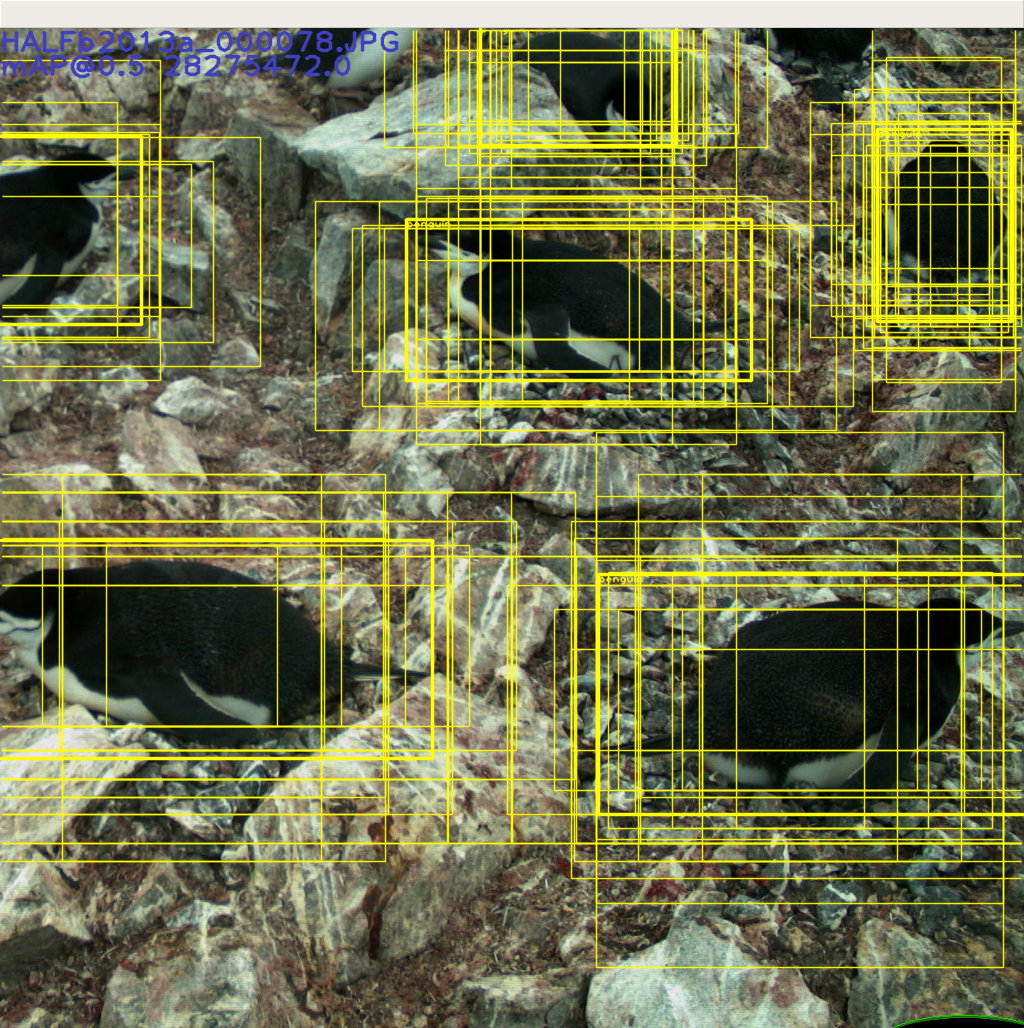
\includegraphics[width=0.95\linewidth]{figures/object/anchors.png}
  \caption{}
  \end{subfigure}%
  \begin{subfigure}[t]{0.30\textwidth}
  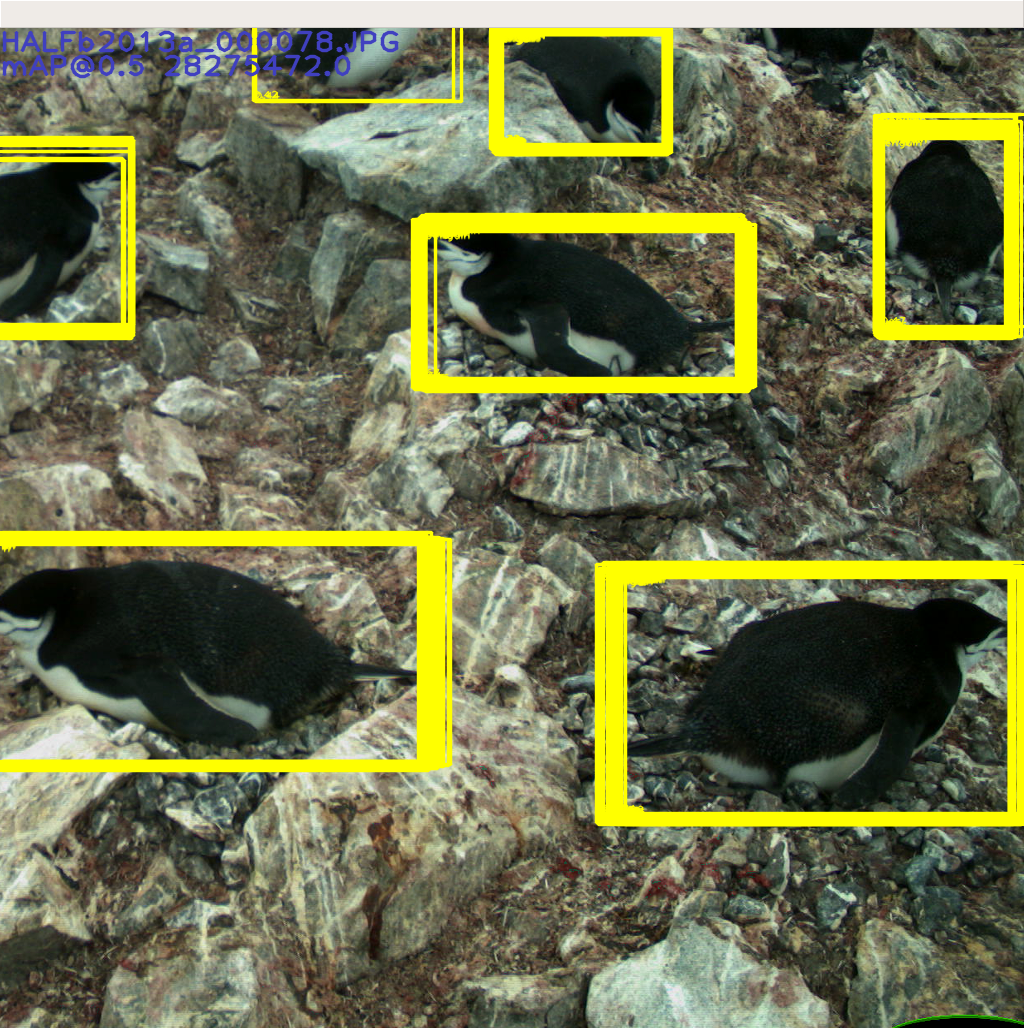
\includegraphics[width=0.95\linewidth]{figures/object/predictions.png}
  \caption{}
  \end{subfigure}%
  \begin{subfigure}[t]{0.32\textwidth}
  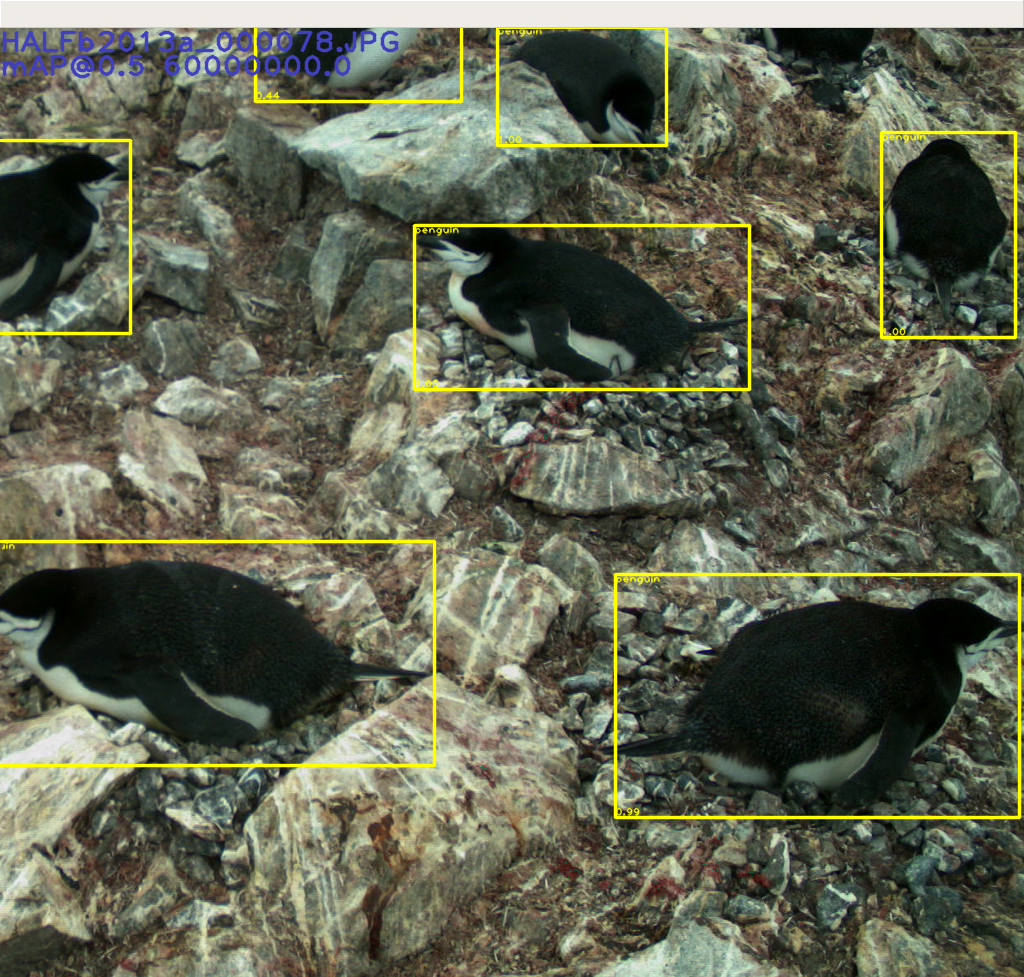
\includegraphics[width=0.95\linewidth]{figures/object/final.png}
  \caption{}
  \end{subfigure}%  
  \caption{Illustration of steps in a single-shot anchor box based object detector: (a) anchor boxes from class predictions (b) refined anchor boxes after transformation (c) final predictions after Non Maxima Suppression.   }
  \label{fig:anchor_boxes}
\end{figure}


I use translation invariant anchor boxes as per \cite{Wang2017}. Anchor boxes are the set of discrete locations and box sizes for which the \gls{CNN} can predict an object exists. It is infeasible to provide a discrete set of boxes large enough to cover all possible object locations; therefore, each anchor box is also modified by a scale and translation (details below in Section~\ref{sec:regression}) to fine-tune anchor boxes to fit objects in the image.

Sets of anchor boxes are used for each level with aspect ratios $ \in \{0.5, 1, 2\} $ and scales $ \in \{2^0, 2^{1/3}, 2^{2/3}\} $. For each feature map at level $k$, with a base scale of $ 2^{k + 2} $ pixels, the set of 9 anchor boxes (all combinations of aspect and scale) are tiled, centred on each feature map pixel. Feature map levels $3$--$7$ are used for object detection giving the smallest (square) anchor at $32\times32$ and the largest at $812\times812$

In training, anchor boxes are selected by matching on \gls{IOU} overlap with ground truth boxes. Each anchor box is matched with the ground truth box with the highest \gls{IOU} overlap. An anchor box matches a ground truth box as a positive if $ IoU >= 0.5 $, anchors with $ IoU < 0.4 $ are treated as negative, and those boxes with $ 0.5 > IoU >= 0.4 $ are ignored (omitted from either positive or negative for computing loss).

Ground truth boxes will match with potentially many anchor boxes, but each anchor box is only assigned to one ground truth box for training.  Overlapping objects with similar position and size may mean that an anchor box which would otherwise have matched, does not (because it more closely matches another object).

\subsection{Total loss function}

The total loss function is defined as a balanced sum between box regression ($L_{loc}$) and class prediction loss ($L_{class}$). 

\begin{equation}
L  = L_{loc} + \lambda L_{class}
\label{eq:loss_total}
\end{equation}

\subsection {Box regression loss}
\label{sec:regression}


I use the anchor box encoding used in \gls{RCNN} \cite{Wang2017} to calculate location loss. The loss is a smooth-L1 loss over regression target ($t^*_x, t^*_y, t^*_w, t^*_h \in t^*_i$) giving a transformation from an anchor box ($a_x, a_y, a_w, a_h$)  to a set of regression targets $t^*_i$ from the ground truth ($g_x, g_y, g_w, g_h$). 

The boxes are encoded as the offset of the centre in both directions (in proportion to the box size) and the log scale of height and width. The encoding of the four targets are given as:

\begin{equation}
\begin{split}
t^*_x = (g_x - a_x) a_w\\
t^*_y = (g_y - a_y) a_h\\
t^*_w = log(g_w / a_w)\\
t^*_h = log(g_h / a_h)\\
\end{split}
\label{eq:encoding_rcnn}
\end{equation}

The localisation loss can be directly computed from these targets and the output of the box prediction sub-network as the sum smooth-L1 regression of $t_i^* - t_i$. Smooth-L1 is a combination of L2 loss near the origin and L1 loss otherwise. It is given as:

\begin{equation}
L_{1;smooth} = 
\begin{cases*}
|x| & if $|x|>\alpha $ \\
\frac{1}{|\alpha|}x^2 & if $|x| \leq \alpha$
\end{cases*}
\label{eq:smooth_l1}
\end{equation}

The commonly used value $\alpha = 0.5$ is used here. The total localisation loss is then summed across matching ($IoU > 0.5$) anchor truth boxes as:

\begin{equation}
L_{loc} = \sum_i{L_{1;smooth}(t_i^* - t_i)}
\label{eq:loss_loc}
\end{equation}

By rearranging the equations,  it is possible to decode bounding boxes from box predictions $t_x, t_y, t_w, t_h$  and an anchor box. These predictions are then in units of pixels and given as the predictions of the object detection network (after a \gls{NMS} process to cull duplicates).

\begin{equation}
\begin{split}
p_x = a_x + t_x  a_w\\
p_y = a_y + t_y  a_h\\
p_w = exp(t_w) a_w \\
p_h = exp(t_h) a_h\\
\end{split}
\label{eq:decoding_rcnn}
\end{equation}

\subsection {Classification loss}
\label{sec:loss}

The experiments use a modified version of the Focal Loss \cite{Lin2017} to handle the class imbalance (negative vs positive) present when sampling anchor box predictions densely.

Focal Loss \cite{Lin2017} reweights the standard \gls{BCE} loss function to deal with a large number of easy negative examples in object detection (the number of unmatched anchor boxes greatly outnumbers the number of matched anchor boxes). Focal Loss enables dense sampling of negative examples present in an image. The standard approach to dealing with the imbalance between positive and negative examples has been to sample the most significant negative examples to provide a fixed positive to negative ratio.

As defined in \cite{Lin2017}, we use the same terminology and variable naming for consistency. The basic two class \gls{CE} equation for binary prediction from the model classifier $p \in \left[0, 1\right]$, and label $y \in \{0, 1\}$  is given:

\begin{equation}
CE(p, y) = 
  \begin{cases*}
  -log(p) & if $y = 1$\\
  -log(1-p) & otherwise\\
  \end{cases*}
\label{eq:cross_entropy}
\end{equation}


The cross-entropy can be rewritten by defining $p_t$ the prediction relative to the given label.

\begin{equation}
p_t = 
  \begin{cases*}
  p & if $y = 1$\\
  1 - p & otherwise\\
  \end{cases*}
\label{eq:class_prob}
\end{equation}

Allowing the \gls{CE} equation to be rewritten more simply:

\begin{equation}
CE(p_t) = -log(p_t)
\label{eq:short_cross_entropy}
\end{equation}


In order to deal with class imbalance, the key idea of \cite{Lin2017} was to reweight the classification loss to be smaller for well classified boxes (small $p_t$) and to be relatively much larger for badly classified boxes (large $p_t$). This was achieved by multiplying the cross entropy by a factor of $(1 - p_t)^\gamma $ with parameter $\gamma$, a sharpening parameter, to give the focal loss:

\begin{equation}
FL(p_t) = - (1 - p_t)^\gamma log(p_t)
\label{eq:focal_loss_p}
\end{equation}

Another way of dealing with class imbalance is to weight one of the classes. A balanced cross entropy loss can then be written by adding a class weighting $\alpha \in \left[0, 1\right]$ the weight for the positive (rare) case in the two-class setting, and an analogous $\alpha_t$:

\begin{equation}
\alpha_t = 
  \begin{cases*}
  \alpha & if $y = 1$\\
  1 - \alpha & otherwise\\
  \end{cases*}
\label{eq:balanced_weight}
\end{equation}

Then the balanced, focused, cross entropy is defined:

\begin{equation}
FL(p_t) = -\alpha_t (1 - p_t)^\gamma log(p_t)
\label{eq:focal_loss}
\end{equation}

I adopt the parameters given in \cite{Lin2017}, using $ \gamma = 2 $, and $ \alpha = 0.25 $. 

The total class loss is then given as the sum of the focal loss computed densely across all classes and anchor boxes in the image (except for anchor boxes between the positive threshold and negative threshold $0.4 <= IoU < 0.5$ which are ignored). For anchor box $i$, $p_i$ is the size $K$ prediction vector from the network, and $p^*_i$ is the size $K$ one-hot target vector. Where $K$ is the number of classes.

\begin{equation}
\begin{split}
L_{class} = \frac{1}{N}\sum_i{\sum_{k \in K}FL(p_{ik}, p^*_{ik})}
\end{split}
\label{eq:total_loss}
\end{equation}

The total loss is then normalised by the number of positive anchor box matches. In this work I use a non-normalised variant of this loss, details described below in Section~\ref{sec:normalisation}.

\subsection{Inference and non-maxima suppression}

In training, a large set of anchor boxes are trained to classify each object detection (those overlapping each anchor box by $0.5$ or more). For the purposes of inference, assigning more than one box for the same object is undesirable, so a greedy \gls{NMS} is used to eliminate multiple detections of the same object. Figure~\ref{fig:anchor_boxes} shows the effect of applying a \gls{NMS} on box predictions: (a) shows the set of boxes classified as containing an object; (b) shows the regressed predictions where many boxes overlap the same object; (c) shows the result of the \gls{NMS}, leaving a single box on each object. In this work a standard \gls{NMS} procedure as per \cite{Wang2017} is used, where boxes are selected from most-confident to least-confident, and boxes overlapping lower confidence boxes by more than an \gls{IOU} threshold (in this work $0.5$) are eliminated.

The use of \gls{NMS} has presented some problems in object detectors, notably the inability to handle highly overlapping objects well. Objects with a high overlap by more than $0.5$ are impossible to detect for such a detector. When used for annotating crowded objects, the inability of the object detector to accurately predict highly overlapping objects means in some datasets the user must spend time correcting artefacts caused by the limitation of the object detector (by no means limited to \gls{NMS}).


\section{Evaluation metrics}
\label{sec:evaluation_metrics}

The most common metric used in object detection is that of \gls{AP}, as popularised by the Pascal VOC challenge \cite{Everingham2008} and later the COCO dataset \cite{Lin2014}. The \gls{AP} is essentially the area under a recall-precision graph for a particular matching threshold and varies from $0$  to $1$. Its primary attraction is that it avoids the need for a detection threshold. It provides a single, relatively easy-to-understand metric which measures precision and recall as well as localisation accuracy (for a particular threshold).

A greedy algorithm finds matches in each image (similar to that used in \gls{NMS} above) where the predictions are matched against ground truth boxes from a most-confident to least-confident order. Each prediction matches its highest overlap ground truth box where the overlap exceeds the \gls{IOU} threshold (amongst ground truth boxes already unmatched). Matches from all images are then merged and sorted by confidence level of the prediction of the match. True-positives ($tp$) and false-positives ($fp$) are found by counting matched and unmatched predictions from high-to-low confidence, and false-negatives ($fn$) are determined at each point by subtracting true-positives from the total ground truth count. 

\begin{equation*}
\begin{split}
p_i = \frac{tp_i}{fp_i + tp_i}\\
r_i = \frac{tp_i}{tp_i + fn_i}
\end{split}
\label{eq:recall_precision}
\end{equation*}

From there, recall ($r$), and precision ($p$) levels can be determined at the confidence level of each prediction. Special cases are added for $r_0=0, p_0=1$ and $p_n=1, r_n=0$, the precision levels are then made monotonic decreasing:

\begin{equation}
\hat{p_i} = \max_{j \in [i..n]}{p_j}
\label{eq:monotonic_precision}
\end{equation}

\gls{AP} can then be calculated by using trapezoid summation:

\begin{equation}
AP = \sum_{i \in [0..n-1]}\frac{\hat{p_i} + \hat{p}_{i + 1}}{2}
\label{eq:trapezoid}
\end{equation}


For multiple class object detection, the metric is usually the \gls{mAP}, defined as the mean of \gls{AP} across classes. This has the effect of making classes have a uniform weight, where there is an imbalanced dataset.  In this work, I use the simpler \gls{AP} instead of the \gls{mAP} as most datasets in this work are single class so, in that case, \gls{AP} and \gls{mAP} are the same. To denote the matching thresholds we use the notation $AP_{IoU}$ or $mAP_{IoU}$. The most permissive matching threshold used is $0.5$ (used as the primary metric for Pascal VOC), and a more strict matching threshold of $0.75$ is often used to measure object detection with precise localisation.

To produce a single metric taking into account localisation accuracy \cite{Lin2014} defined a metric COCO \gls{AP} as the mean of \gls{mAP} at a series of matching thresholds $ IoU \in [0.5 : 0.05 : 0.95] $, confusingly this mean-\gls{mAP} is often termed just \gls{AP}. In this work, I refer to $AP_{COCO}$ as the average of the $AP_{IoU}$ across this range (instead of the $mAP$) as is usual in the multi-class setting.

\begin{equation}
AP_{COCO} = \frac{1}{10}\sum_{i \in [0.5 : 0.05 : 0.95]}AP_{i}
\label{eq:ap_coco}
\end{equation}

There are downsides to the \gls{AP} family of metrics. The precision-recall graph created using decreasing confidence considers only the order of detection confidence. This has implications in that the level of false-positives which occur at lower confidence than the last true-positive are ignored. In addition, the margin between confidence levels is ignored, so the sensitivity to change in confidence levels is not taken into account. The threshold on \gls{IOU} overlap also means that all true-positives which meet the localisation threshold are treated equally. Those which match the ground truth perfectly are scored the same as those which meet only the minimum match threshold. Alternatives exist, although arguably not as easy to understand as \gls{AP}, for example \cite{Oksuz2018}, which tries to weight true-positives for localisation accuracy, as well as attempting to provide a way to determine the ideal detection threshold.


\section{Proposed methods}
\label{sec:object_methods}

In this section I outline the key differences between the object detection method this work is based on, RetinaNet \cite{Lin2017}, and outline proposed modifications for the purposes of image annotation.

\subsection{Network architecture}

The object detection models bear a close similarity to the segmentation models discussed and used in Chapter~\ref{chap:bootstrap}, such as UNet \cite{Ronneberger2015}. \gls{FPN} models utilise shortcut connections in the same way, the significant difference from segmentation models being that anchor boxes are predicted at multiple levels of scale, where segmentation models output mask predictions only at one resolution.


\begin{figure}[htb!]
  \centering
  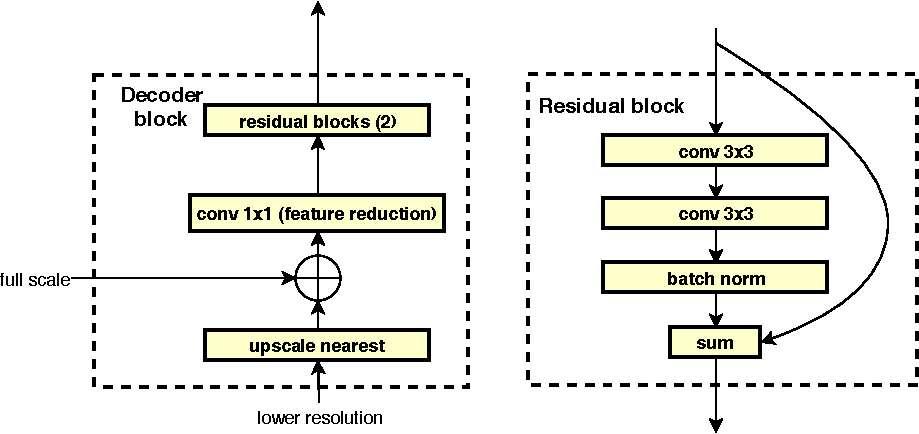
\includegraphics[width=1.0\linewidth]{figures/annotation/decoder_block.pdf}
  \caption{Decoder block, responsible for merging half-resolution features with features from full-resolution skip connections }  
  \label{fig:decoder_block}
\end{figure}


\begin{figure}[htb!]
  \centering
  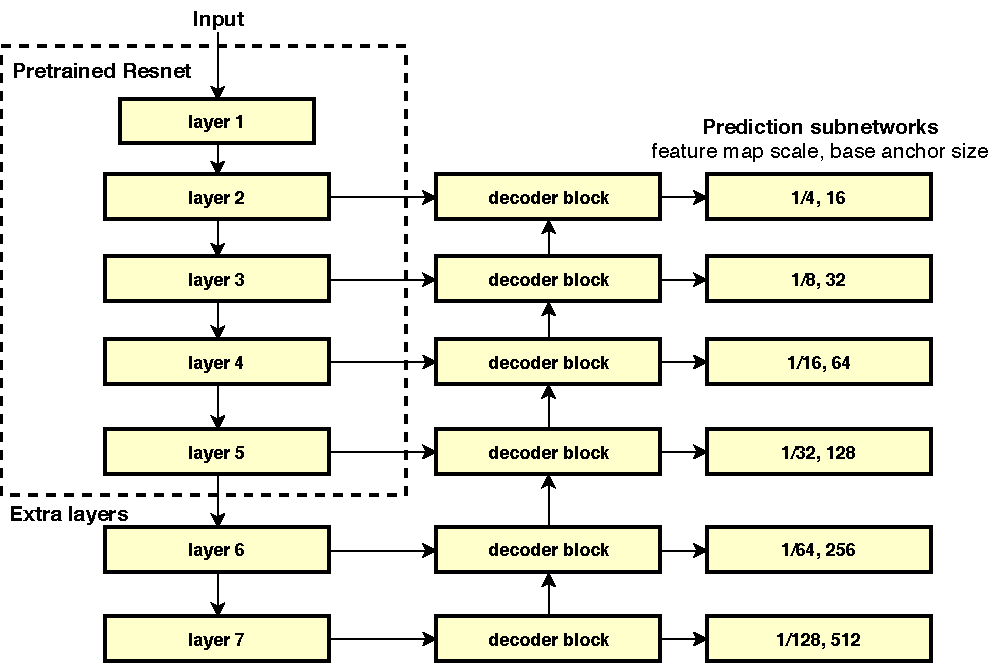
\includegraphics[width=1.0\linewidth]{figures/annotation/detection_network.pdf}
  \caption{Object detection network, built on the backbone ResNet }  
  \label{fig:detection_network}
\end{figure}

\begin{figure}[htb!]
  \centering
  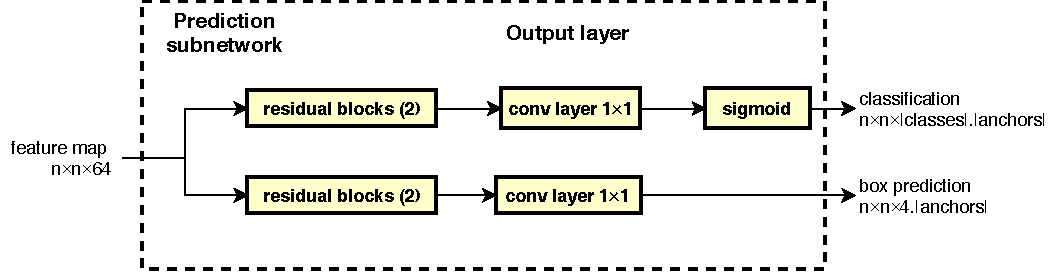
\includegraphics[width=1.0\linewidth]{figures/annotation/prediction_subnet.pdf}
  \caption{Prediction sub-network with two streams, one for classifying anchor boxes with one output per class for each anchor box, the other stream for location regression for each anchor box (shared between classes)}    
  \label{fig:prediction_subnet}  
\end{figure}


Some parameters and network architectures differ from \gls{FPN} \cite{Lin2017a}. For the most part, the modifications are small things which seem to enable it to learn better on small datasets used for experiments in this work. These include adding extra residual layers to the decoder, shown in Figure~\ref{fig:detection_network}. It is more similar to the network shown in Chapter~\ref{chap:bootstrap} than the \gls{FCN} network. A key difference is that neither the weights between classification sub-networks nor box regression subnets are shared between different scales  (RetinaNet shares weights between classification sub-networks). I found in the small scale datasets used in this work that shared weights on the class sub-network significantly slows initial learning. The extra residual layers in the decoder side of the network (Figure~\ref{fig:decoder_block}) improved this significantly, but not entirely. 



\subsection {Non normalised loss}
\label{sec:normalisation}

In \cite{Lin2017}, and Equation~\ref{eq:total_loss} a normalisation occurs over the total loss by the total number of positive matching anchor boxes, in order to average the error from the positive targets. This assumes the contribution from negative targets is either negligible or roughly proportional with the number of positive targets.

In order to allow training on purely negative images, it is necessary to avoid a division by zero. One method is to add a constant to the denominator, representing the contribution of the negative classification targets; the other is not to normalise. I experimented a little with both options, finding them to be reasonably robust. The experiments in this work use the non-normalised class classification loss.
One aspect that was noticed in the implementation of the segmentation tool from Chapter~\ref{chap:bootstrap}, was that the original images were often much clearer than the scaled down images (for a human annotator to see fine details), with clarity being lost at lower resolutions. 

\subsection{Training and inference on high-resolution images}
\label{section:high_res}

High-resolution images present a cost in terms of training (and inference) time, and also in terms of the memory and data required to transfer over a network. High-resolution images are undoubtedly easier to annotate, as small details become apparent, whereas scaled down images often obscure details and as a result make the annotation task ambiguous. It is not necessary to feed the model images at the same resolution as the user annotates, but if a human annotator has trouble with ambiguity due to a reduction in resolution, it seems a reasonable assumption that a \gls{CNN} will too, especially for datasets with many small examples. The datasets used here (see Chapter~\ref{chap:annotation} for details), contain many small objects and many objects with a high degree of uncertainty and ambiguity.

With that in mind, I focused on preserving resolution for the annotation process as it is hypothesised the benefits outweigh the drawbacks. In Section~\ref{sec:scale_crop}, I experimentally validate this idea by comparing training with different resolutions (and crop sizes) for a selection of datasets.

In object detection datasets, larger objects have consistently been shown to be easier to detect (having a higher accuracy than medium or small objects) \cite{Lin2014, Wang2017, Lin2017a, Law2018, Zhou2019}. The COCO dataset defines \emph{small} as having an area of $<32^2$ and \emph{large} having an area of $>96^2$ pixels. In addition, detectors trained at higher resolutions on the same datasets consistently show higher performance. When trained at a high-resolution, the number of objects considered to be \emph{large} by the COCO definition is significantly increased.

 Compared to the PASCAL VOC \cite{Everingham2008}, or COCO \cite{Lin2014} datasets which have a broad range of scales, in the majority of data experimented on in this thesis, the objects of interest occupy an area much smaller than the total image size. An analysis of object sizes of two of the less extreme datasets compared to VOC and COCO can be seen in Figure~\ref{fig:box_sizes}. 
 
\subsubsection {Training method}
\label{sec:highres_inference}
 
I propose that it is possible to get away with larger image sizes by using smaller crops of the original images to train, as long as the objects fit in the image crops. I do some experiments on this idea in Section~\ref{sec:experimental_validation}, in order to test this hypothesis where I compare training at different image scales and crop sizes. The method of crop selection is described in Section~\ref{sec:preparation}. 

For very large objects, where objects may be larger than any reasonable crop size I would propose a multi-scale inference (and a wider range of training scales). None of the datasets annotated in this work had sufficiently large objects to necessitate this.

Use of simpler, faster models has been successful as the backbone of the object detection network (for example, ResNet-18 \cite{He}), which enables larger images to be used in both training and evaluation. Time taken for evaluation and training is also much improved, relative to using larger networks. For the smaller datasets in our experiments, I did not see significant improvements in accuracy when using larger backbone networks.


\subsubsection{Inference methods}

I looked at two different possibilities for performing inference on a full-resolution image using an object detector network trained only on crops of images: (a) pass in the full image using the property that the network is \emph{fully convolutional} and (b) tile images the same size as training crops and collapse the predictions using a combined \gls{NMS}. In order to facilitate this idea, the box annotations on the edge of images are estimates of the full bounds of the object, and the anchor boxes are not cropped to the edge of the image. In \cite{Duarte2010}, the approach of annotating the estimated full bounding box (the approach I have taken) was compared to annotating just the visible parts (as is more common practice) in a pedestrian detector. Estimating the full bounds was a slight improvement, however, the fusion of both was found to be better than either one. 

The first method is to pass in the full image to the neural network, even though it has only been trained on much smaller crops. Object detection networks are flexible and work across a range of input image resolutions. All layers are either convolutions or do not reshape the feature maps (aside from up/downsampling). As a result, passing in a larger image results in a larger feature map and set of box outputs at each layer of the pyramid. The concern is that the up/downsampling behaviour is slightly different for input sizes depending on if they are odd or even, relative to powers of two. I found this to be a legitimate concern, though largely negated if the training crop size is set to a power of two or multiple of a power of two. 

The second inference method is to tile multiple inferences at the size the model was trained at, across the full image size, using a certain overlap buffer region. The result is sets of overlapping predictions at the edges. These overlapping predictions can be decimated using a combined \gls{NMS} so that it removes duplicates overlapping from two adjacent tiles. The concern with this method is that edge detections are possibly inaccurate and may produce erroneous predictions which are not removed by \gls{NMS} because of their inaccurate localisation. 

Image size has its limits for both training and inference, as the complexity of the model and the size of the memory on the \gls{GPU} determines the maximum size image which can be processed. I can process the large images used in this work because of the relatively simple backbone model used (ResNet-18 \cite{He}). Evaluation using tiling makes it feasible to use larger image sizes and more complicated models, even if multiple inferences take more time.

\subsection{Small object sizes and circle annotations}
\label{sec:small_object}

In \cite{Lin2017}, feature maps on levels $3$--$7$ are used for object detection. Giving the smallest (square) anchor at $32\times32$ and the largest at $812\times812$. In the case of datasets with very small objects (datasets \emph{scott base} and \emph{penguin survey}), anchor boxes on level 2 are added, which provide anchor boxes as small as $16 \times 16$, allowing more precise localisation of very small objects.

In the case of counting, a box is not necessary and takes longer to input than to use a circular annotation. Where circles are used for annotation, just three anchor boxes are used, with only the square aspect ratio used at each scale. For all intents and purposes, the circles with radius $r$ are treated as a square box with side lengths $2r$, and the box regression sub-network is modified to produce only $3$ outputs (enforcing square aspect ratio for height and width).


\subsection {Cyclical learning rates}
\label{sec:schedule}

\begin{figure}[htb]
  \centering
  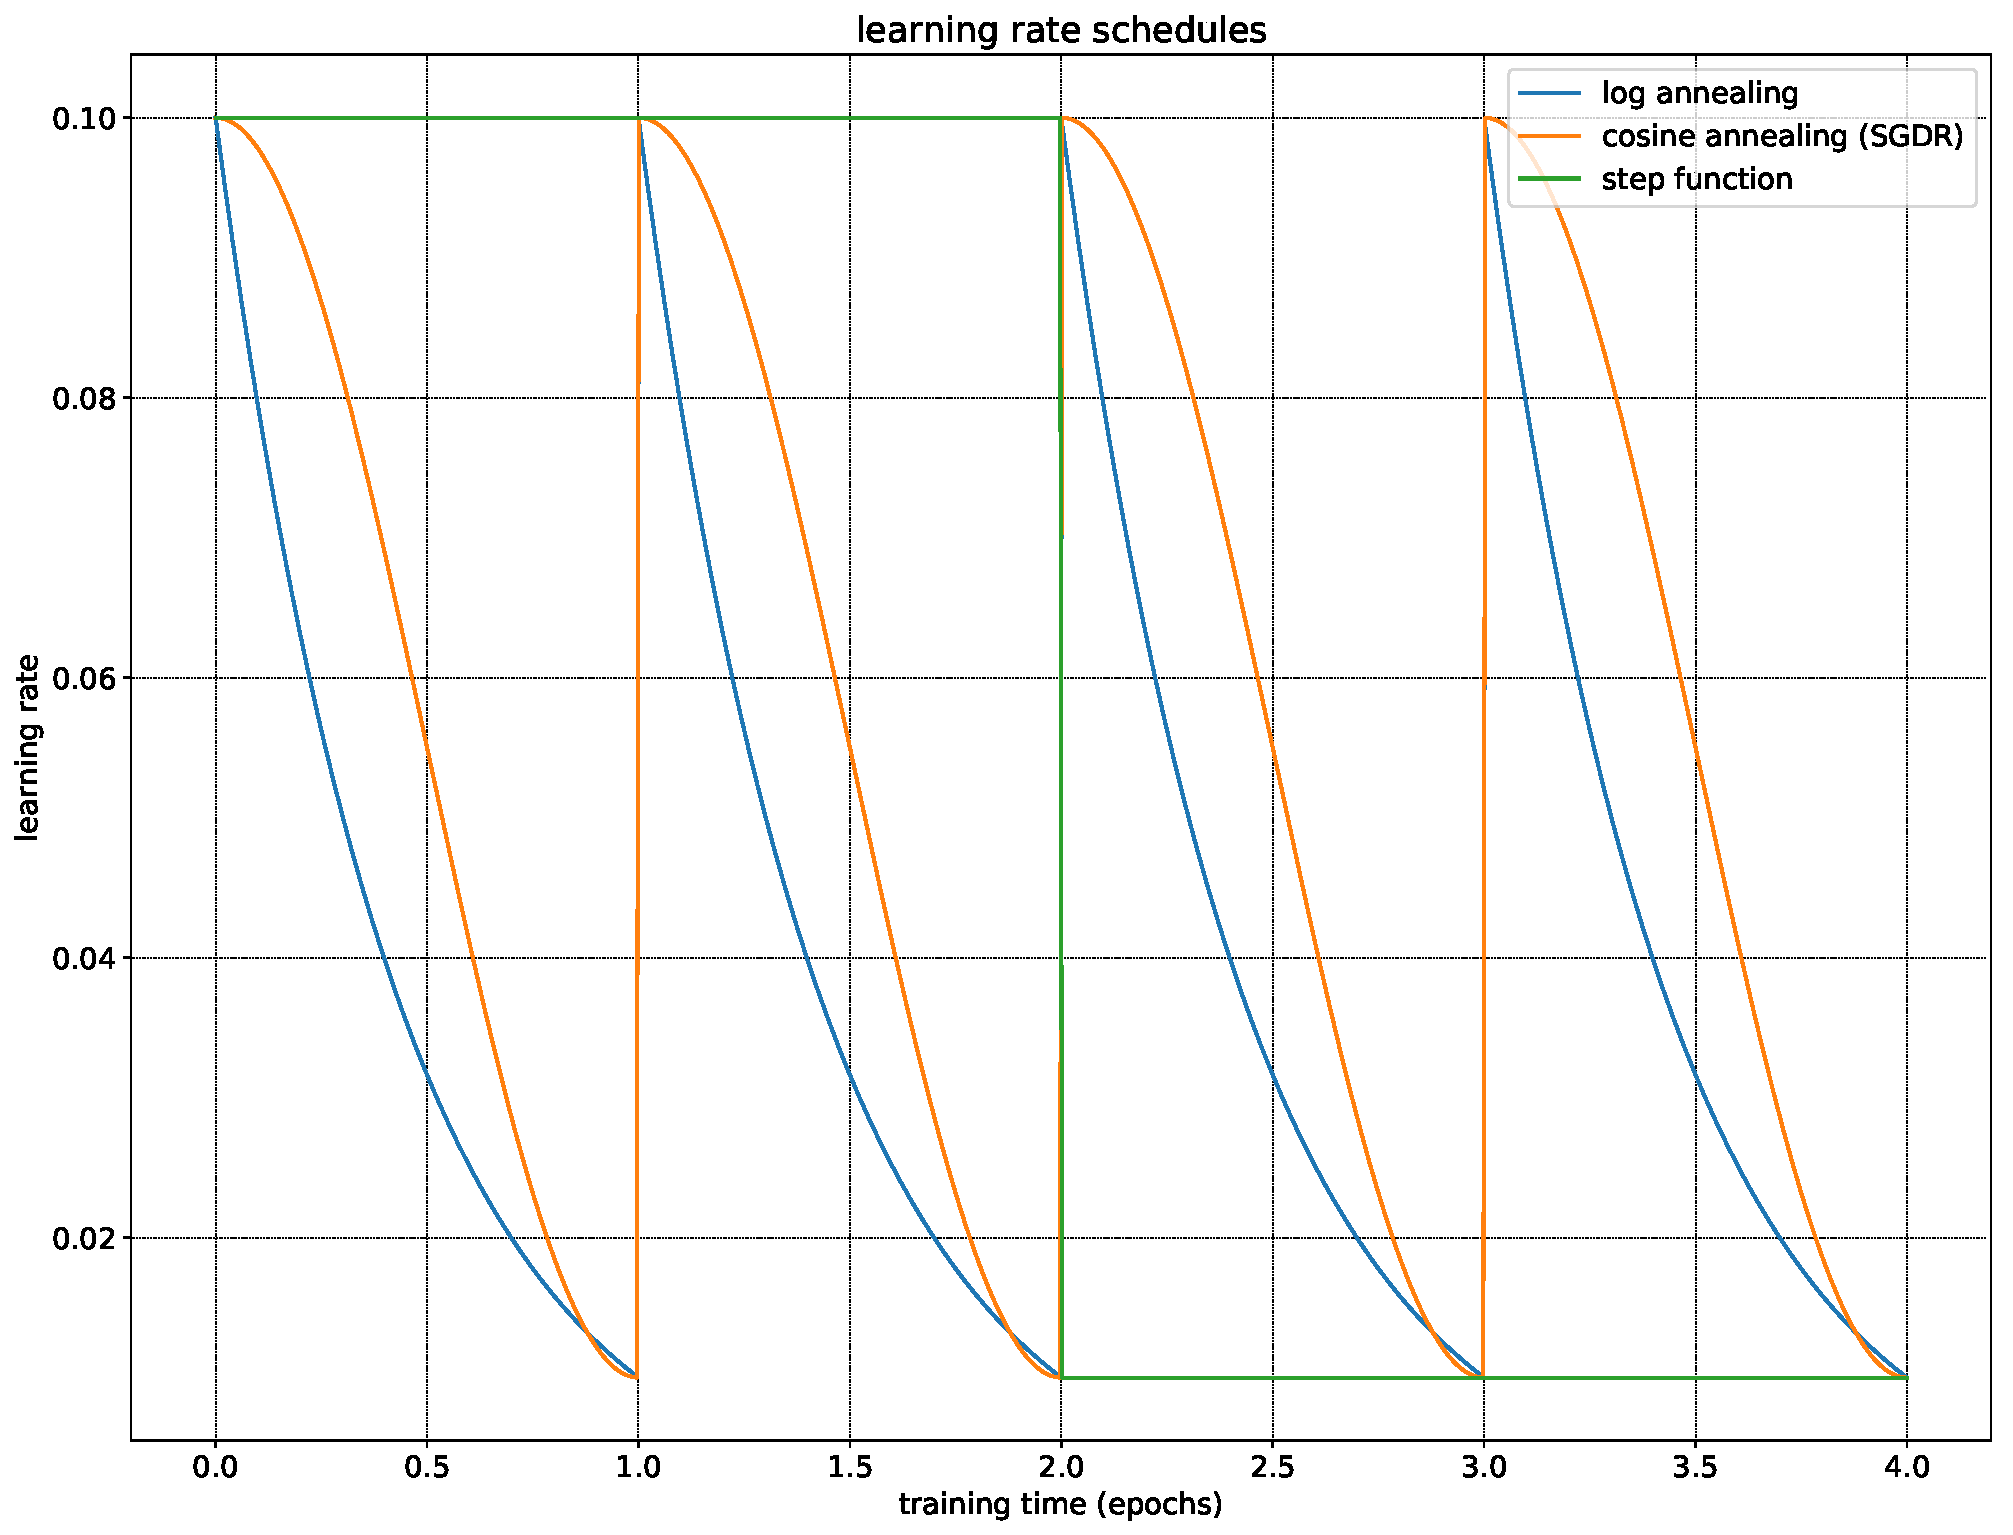
\includegraphics[width=1.0\linewidth]{charts/training/lr_schedules.pdf}
  \caption{Comparison of learning rate schedules, cyclical learning rates and traditional step function.  }  
  \label{fig:lr_schedule}
\end{figure}

In order to facilitate continuous online learning, where examples are added over the training lifetime, a cyclical learning rate and relatively short learning epochs are used. The idea is that a large learning rate is used for a short period to incorporate information from newly annotated examples, then the learning rate is reduced for a \emph{fine-tuning} in order to use the model for inference.

Epochs are set at a fixed size ($1024$ unless otherwise specified), using uniform random sampling. Learning rates are set for each batch, reducing over an epoch by a factor of $10$, using logarithmic annealing shown in equation~\ref{eq:log_annealing}. Where $base$ is the base learning rate, and $ t \in [0, 1) $ is the progress across an epoch.

\begin{equation}
lr_{log}(t) = exp(ln (lr_{min}) (1 - t) + ln(lr_{max})  t)
\label{eq:log_annealing}
\end{equation}

For comparison, the learning rate schedule used in \gls{SGDR} \cite{Loshchilov2016}, has more weight on the highest and lowest learning rates but is otherwise similar.

\begin{equation}
lr_{cos}(t) = lr_{min} +  \frac{1}{2} (lr_{max} - lr_{min}) (1 + cos (t \pi))
\label{eq:cosine_annealing}
\end{equation}

A comparison of the cyclical learning rates compared to a standard learning rate step schedule is shown for an $8$ epoch training schedule in Figure~\ref{fig:lr_schedule}.

\section{Training details and parameters}
\label{sec:training_parameters}

In this section I attempt to bring together training parameters, not discussed elsewhere, in one place for simpler reference.

\subsection {Image preparation and augmentation}
\label{sec:preparation}

\begin{table}[h]
  \centering
    \caption{Ranges of parameters used for image augmentation; translation occurs as part of a cropping process}
    
  \begin{tabular}{ l  l }
    parameter & range \\
    \toprule
    scale (log uniform) & ${3/4}$--${4/3}$  \\ 
    aspect scale (proportion)  & $ 1 \pm 0.1 $  \\ 
    brightness adjustment (additive) & $ \pm 10 $ \\ 
    contrast (multiplicative) & $ 1 \pm 0.1 $ \\
    gamma adjustment & $ 0 \pm 0.1 $ \\ 
    hue shift & $ \pm 5 $ \\ 
    saturation shift & $ 0 \pm 5 $ \\ 
    horizontal flips (probability) & $ 0.5 $ \\ 
    
    \bottomrule
  \end{tabular}
\label{tab:obj_augmentation}
\end{table}

A region is cropped from the image (using the crop selection method described below), that region is then scaled to the standard training size (denoted as $crop$ below). Photo-metric distortion with parameters from Table~\ref{tab:obj_augmentation} and image whitening is applied. Image whitening is used to ensure consistency with ImageNet trained models (used as the backbone of the object detection network) subtracting mean (r, g, b) $ (0.485. 0.456, 0.406) $ and dividing by standard deviation $ (0.229, 0.224, 0.225) $.

\subsubsection{Crop selection}

First, a size ($size_w, size_h$) and aspect ratio $aspect$ is selected by taking a random value from the valid range of scales, and aspect ratios. I use a geometric uniform random value, where the lower bound is referred to as $scale_l$, and the upper $scale_u$. $\mathcal{U}$ is the uniform distribution over a certain range.

\begin{equation}
\begin{split}
    s \sim \mathcal{U}(\log scale_l, \log scale_u)\\
    aspect \sim \mathcal{U}(\log aspect_l, \log aspect_u)\\
    size_w = crop \cdot e^s \cdot \frac{1}{\sqrt{aspect}} \\
    size_h = crop \cdot e^s \cdot \sqrt{aspect}
\end{split}
\label{eq:random_crop}
\end{equation}

Secondly, a centre point is selected in one of two ways (selected at random with equal probability). One by centring on an object instance chosen uniformly at random between all object instances in an image. The other by selecting a random centre point at random by taking a random centre point $c_x$, $c_y$, In both instances the resulting point is clamped to be within the valid image region $c_x \in [size_w, width - size_w]$, $c_x \in [size_h, height - size_h]$

\begin{equation}
\begin{split}
    c_x \sim \mathcal{U}(size_w - border, width + border - size_w)\\
    c_y \sim \mathcal{U}(size_h - border, height + border - size_h)\\
\end{split}
\label{eq:random_crop2}
\end{equation}

The reason to expand the selection region by a border is that the border pixels always occur less frequently, and often border pixels in images contain different content, for example text such as the date and time or effects from fish-eye distortion removal. Without this border expansion, artefacts often arise during inference as a result of the special content around image edges. 

In the case where the $size$ selected is larger than the input image, an output image at that size with pixels set to the ImageNet mean $ (0.485. 0.456, 0.406) $ and the input image is placed at a random position within the image.


\subsection {Training parameters}
\label{sec:parameters}

\subsubsection{Scale and crop size}

Experiments in Section~\ref{sec:experimental_validation} refer to a scale factor, where the input images are scaled by a factor. The purpose of this scaling is either for testing the effectiveness of high-resolution images (Section~\ref{sec:scale_crop}), or for accelerating the running of validation experiments because to achieve the quantity of experimentation otherwise would take far too long.

In each case the crop size is specified in terms of the original image at $100\%$ size, therefore if the scale is set to $0.5$, the image size used in training is half of the stated crop size, in pixels.

The crop sizes used in experiments and in image annotation, are specific to each dataset and can be seen in Table~\ref{tab:resolutions}, ranging from $1024\times1024$ for many of the high-resolution datasets such as $apples^1$ and $seals$, down to $320\times320$ for the \emph{branches} dataset.

\subsubsection{Optimiser}

In all experiments in this work I use a \gls{SGD} optimiser with the learning rate set to $0.001$, momentum $0.9$ and weight decay $0.0001$ in all cases. Total loss is averaged across each mini-batch, and batch sizes of $8$ are used. The balance factor between localisation and classification loss is $\lambda=2.5$ in all cases.

In Chapter~\ref{chap:bootstrap} much attention was placed on fine-tuning, where the weights of the backbone network used a lower learning rate. For object detection it made little difference; if anything it just made training slower, so it was not used.


\section {Experimental validation}
\label{sec:experimental_validation}

In this section, I evaluate a number of the assumptions and design choices for the object detector.

\subsection {Effect of image resolution and crop size}
\label{sec:scale_crop}

For this experiment I vary the scale and crop size to test the idea that an high-resolution object detector can be trained on small parts of images, then the whole image used in inference.

\begin{figure}[htb]
  \centering
  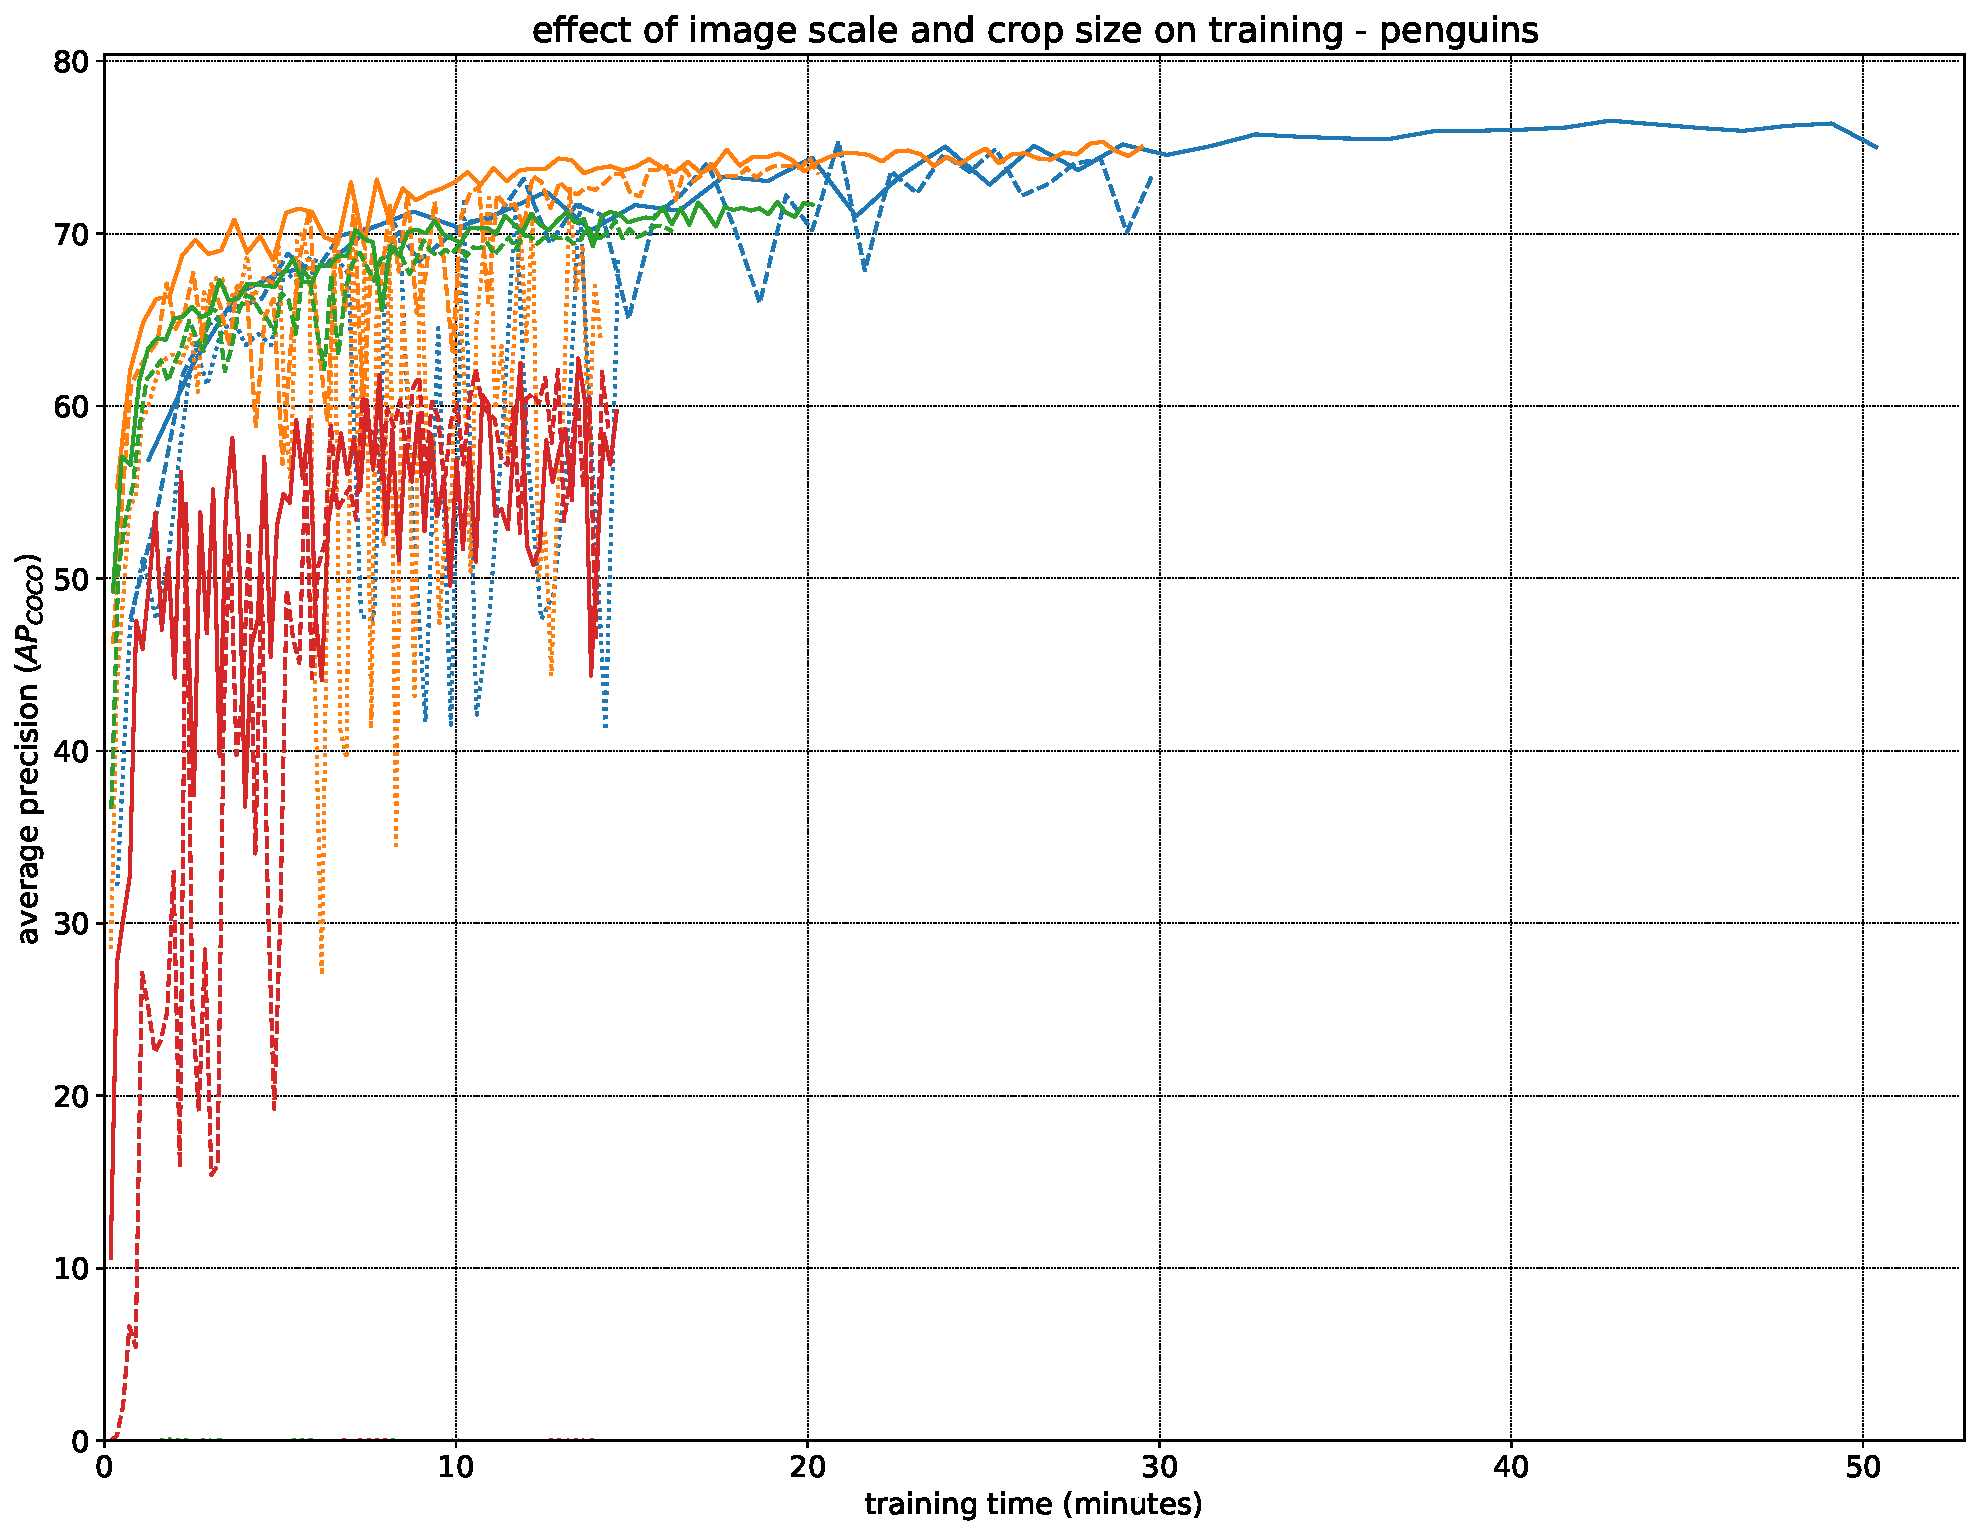
\includegraphics[width=1.0\linewidth]{charts/training/crops_scales/penguins.pdf}
  \caption{Comparison of training at different crop size:scale for $apples^1$ dataset. }  
  \label{fig:apples_crop_scale}
\end{figure}

 
\begin{figure}[htb]
  \centering
  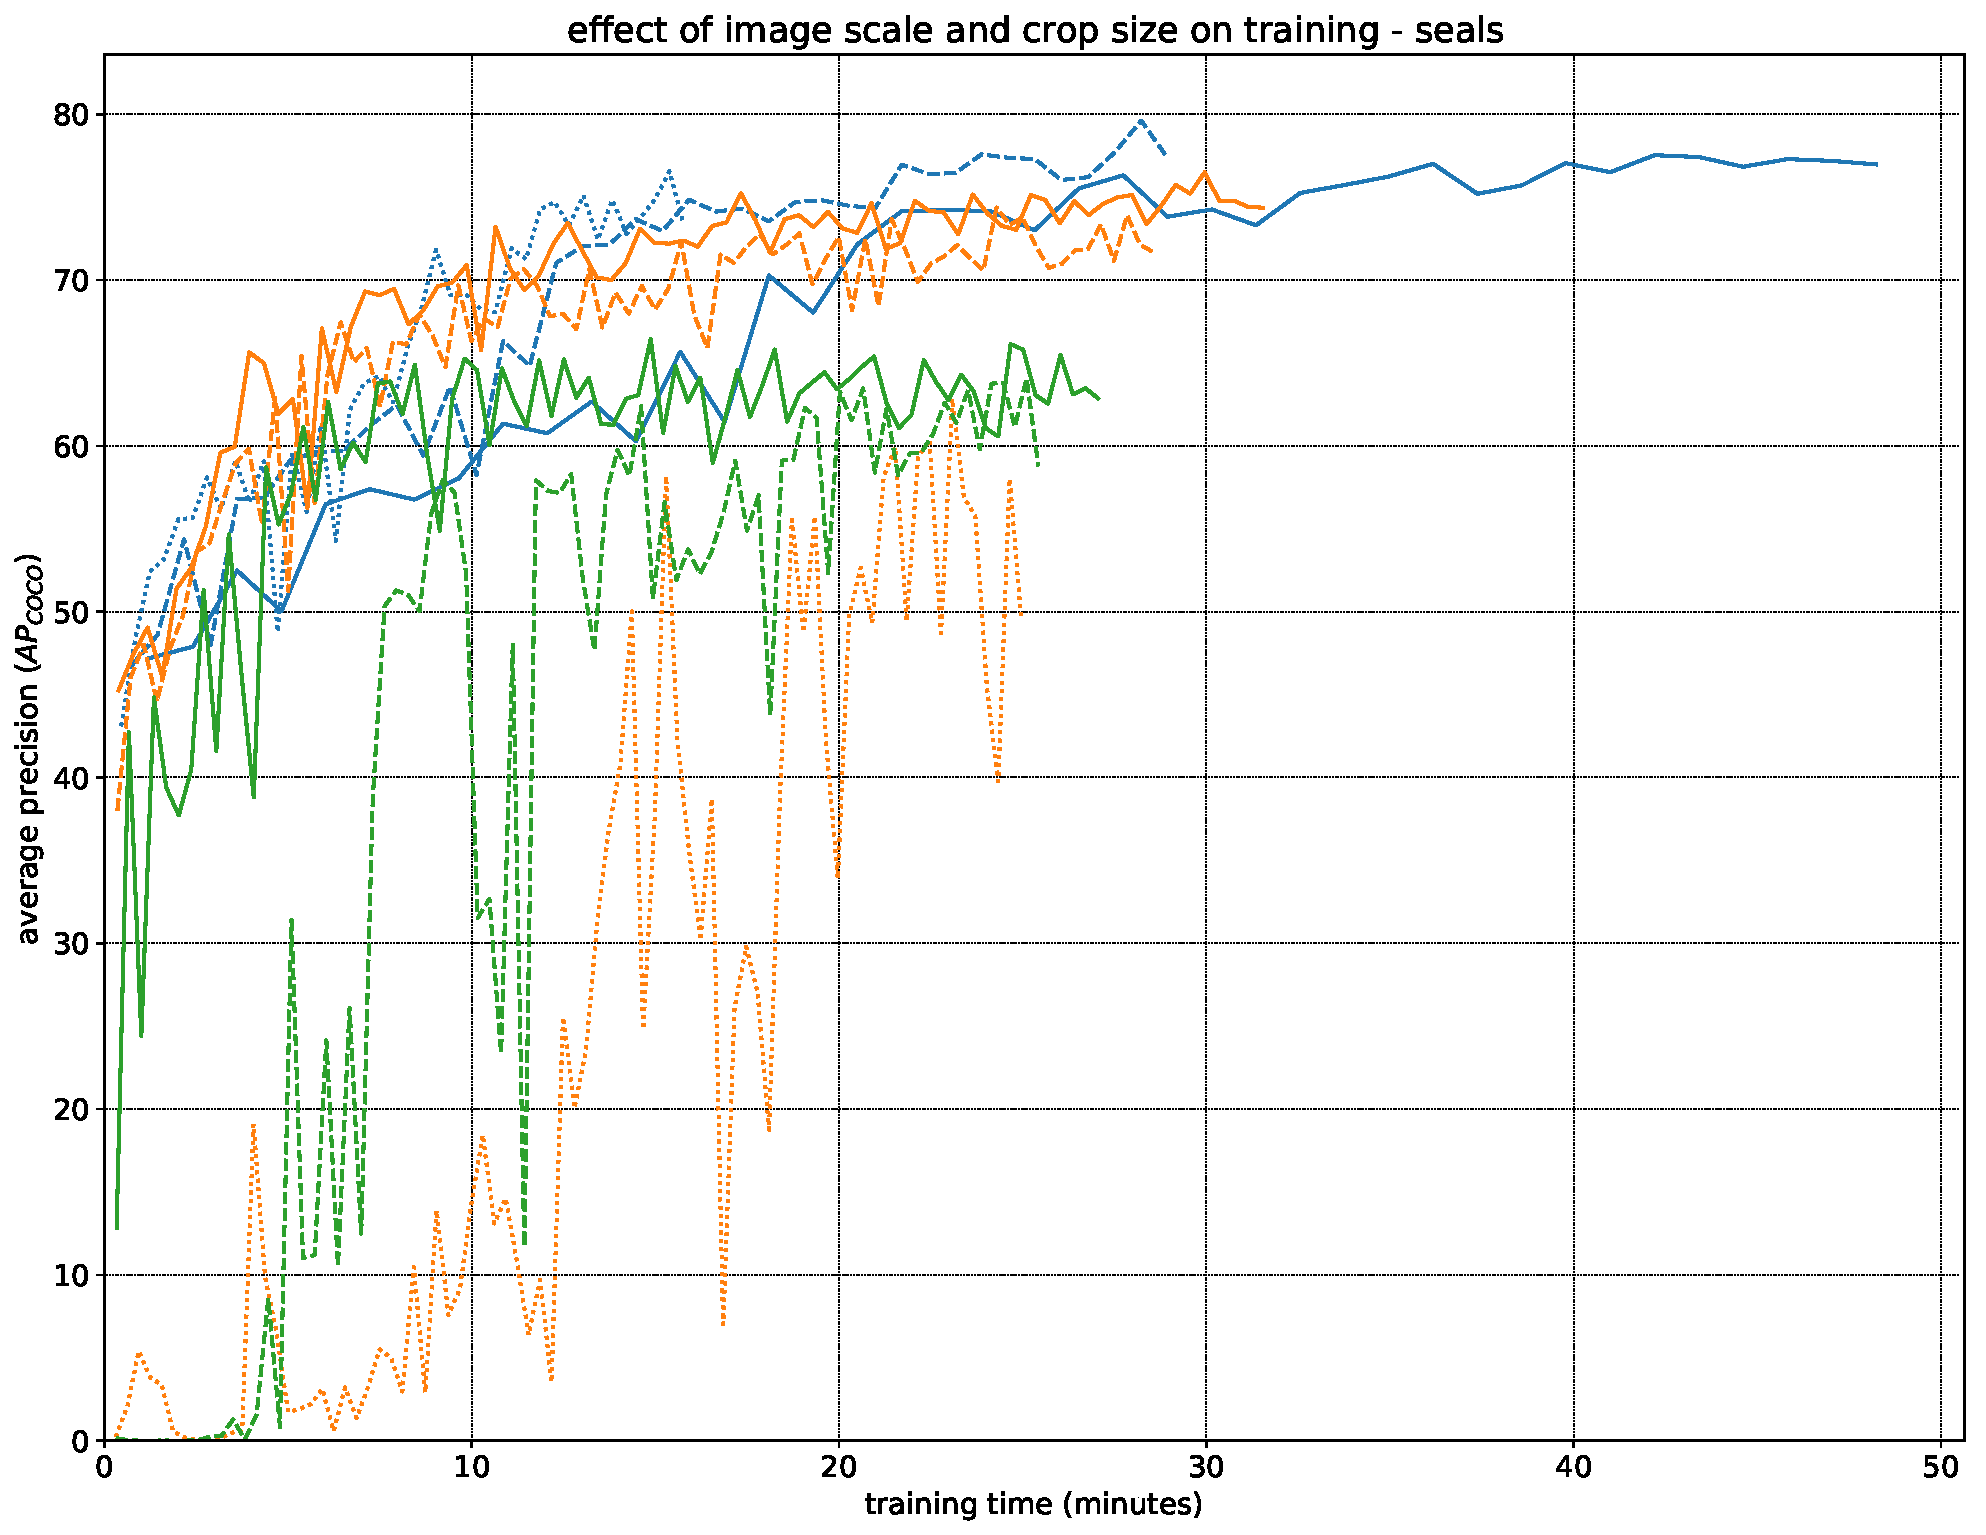
\includegraphics[width=1.0\linewidth]{charts/training/crops_scales/seals.pdf}
  \caption{Comparison of training at different crop size:scale for \emph{seals} dataset. }  
  \label{fig:seals_crop_scale}
\end{figure}


\begin{table}[hbt!]
  \centering
    \caption{Effect of scale and crop size on validation accuracy (percent of best $AP_{COCO}$). Average across datasets ($apples^1$, \emph{penguins}, \emph{scallops}, \emph{seals}) }
    
  \begin{tabular}{ l l | l l l l}
    & scale & 12.5\% & 25\% & 50\% & 100\% \\
    \toprule
       \multirow{2}{*}{\STAB{\rotatebox[origin=c]{90}{crop}}}
       & 512   & 0.0  & 2.4  &  59.3  & 82.8 \\
       & 768   & 17.4 & 68.2  &  90.0 &  96.4 \\
       & 1024  & 28.5 & 81.9  &  95.0  & 100.0 \\
    \bottomrule
  \end{tabular}
\label{tab:accuracy_scale_crop}
\end{table}

Full-resolution provides the best accuracy, although, in many of the datasets half-resolution provided almost the same accuracy while providing much faster training and inference. At half-resolution, an ensemble could be trained in a similar time to training one network at full-resolution and used to provide uncertainty measurements. On the other hand, as seen below in Section~\ref{sec:lr_schedule_exp}, the training accuracy is limited by the size of the dataset more than the training time. Training time is severely dependent on human annotation time, which will allow plenty of time for training at high-resolution.

The training speedup is measured, but note the figure for training time is just the training time, and excludes time for validation. It would be expected that halving the image resolution would halve the training time, but that figure is instead a speedup factor of $3.3$. The reason for that is that the images are loaded at full-resolution, so the bottleneck becomes the image loading and could be easily alleviated by resizing the images in advance.

\begin{table}[hbt!]
  \centering
    \caption{Speedup associated with reduced resolution. Average across datasets (\emph{apples}, \emph{penguins}, \emph{scallops}, \emph{seals})  }
  \begin{tabular}{ l l | l l l l}
    & scale & 12.5 & 25 & 50 & 100 \\
    \toprule
       \multirow{2}{*}{\STAB{\rotatebox[origin=c]{90}{crop}}}

        & 512   & 6.0  & 5.9  &  5.9  & 3.3 \\
        & 768   & 5.9 & 5.3  &  4.4 &  1.7 \\
        & 1024  & 5.9 & 4.5  &  3.3  & 1.0 \\
    \bottomrule
  \end{tabular}
\label{tab:speed_scale_crop}
\end{table}


Using a larger crop size proved more accurate in all of the four datasets, and using a larger crop was beneficial in all cases, being more accurate and more stable to train. The larger size, however, trains much more slowly, so in an active learning system, it is possible to use the time savings for other things such as evaluating unseen images for example selection or training a set of several models to use as an ensemble.


\subsection {Inference method for large images}

\begin{figure}[htb] 
  \centering
  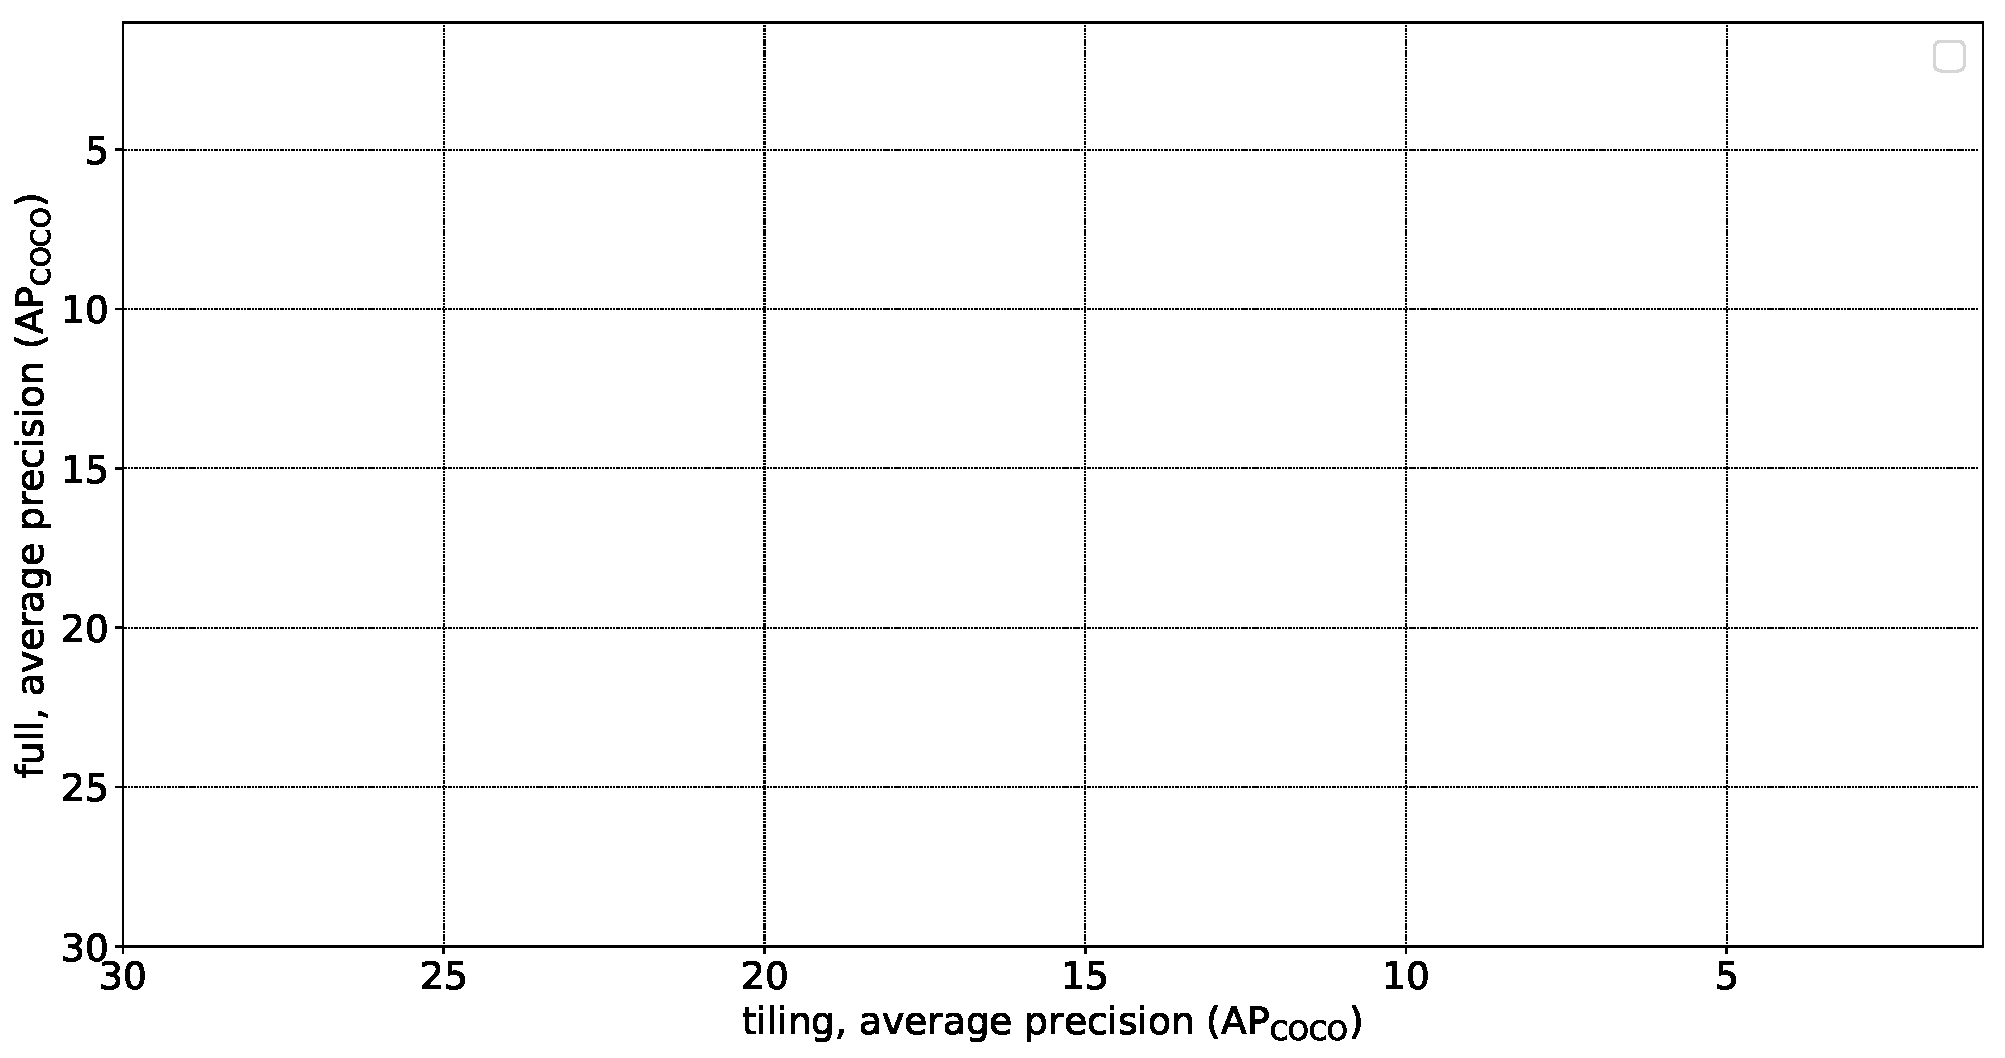
\includegraphics[width=1.0\linewidth]{charts/training/splits_scatters.pdf}
  \caption{Comparison of different inference methods across one training run with inference using tiling vs. inference on full images. Training occurs on crops and evaluating on full images. }   
  \label{fig:inference_method}
\end{figure}


I compared the two methods (tiling vs inference on the full image) by using both methods for testing against the validation set of several different training runs. It can be seen in figure \ref{fig:inference_method} that both perform very similarly. Sometimes one is marginally better, and sometimes the other is marginally better, even within the same training run.

\subsection{Incremental learning}
\label{sec:incremental_learning}

\begin{figure}[!p]
  \centering
  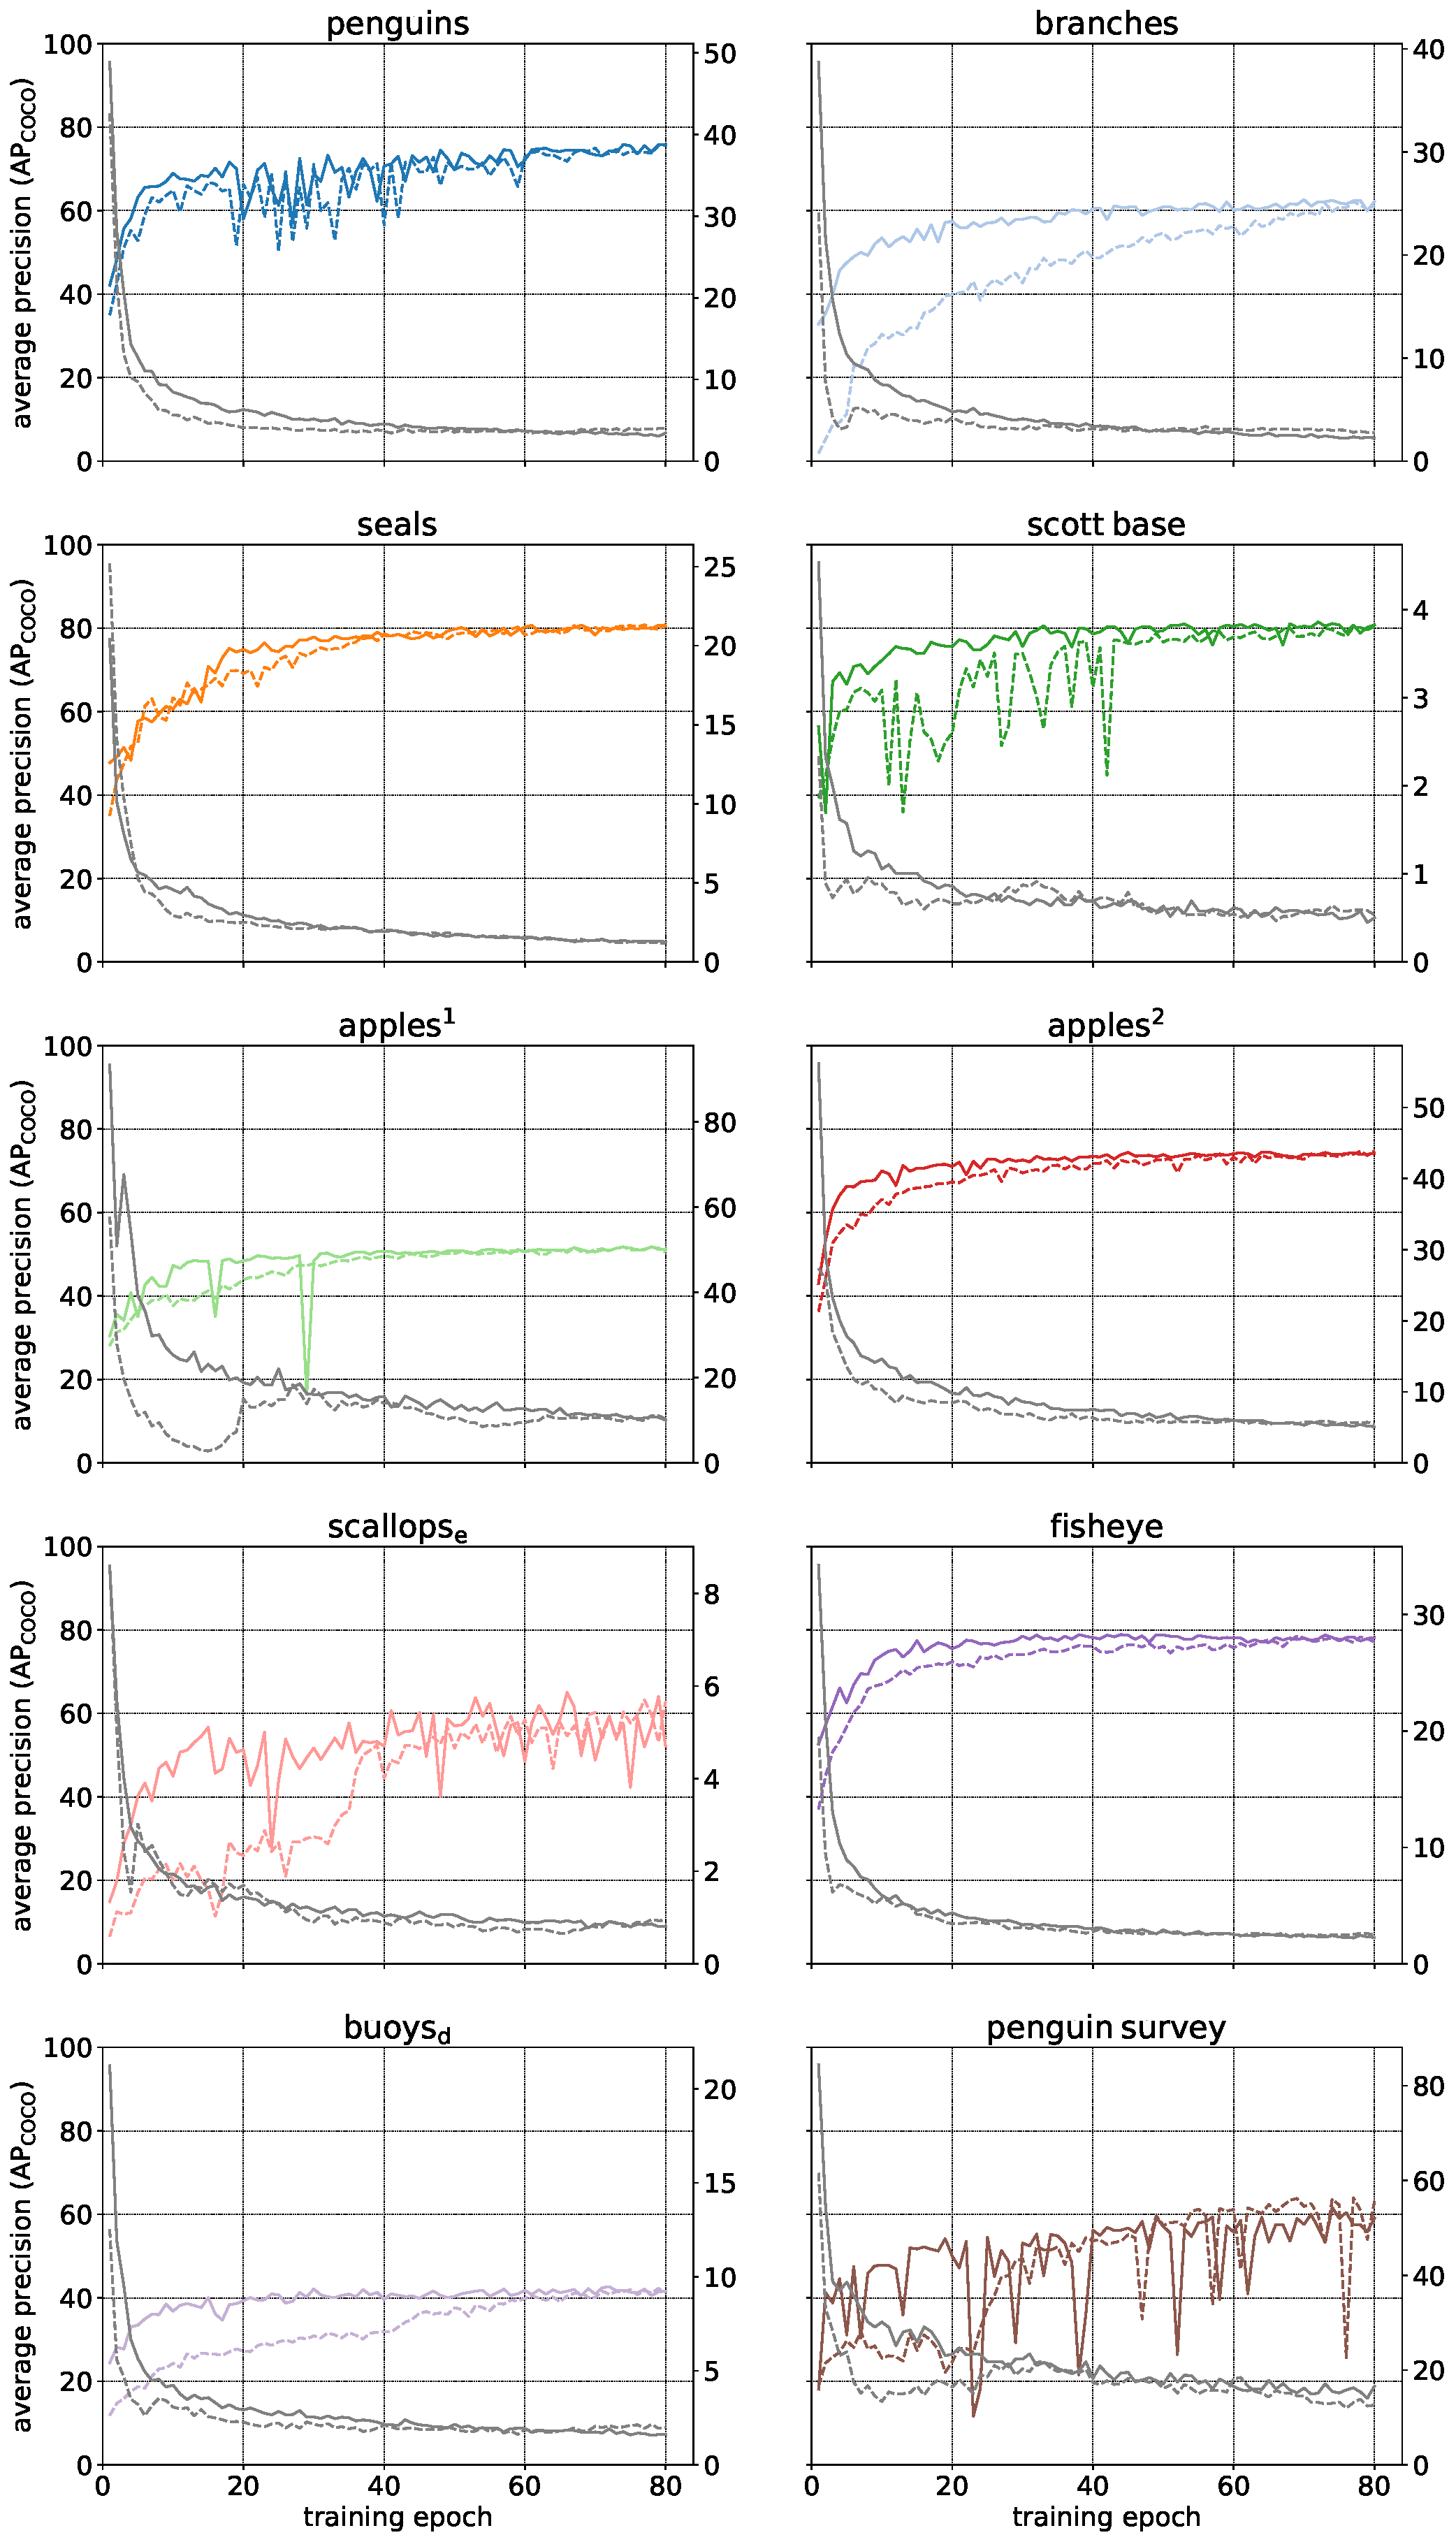
\includegraphics[width=0.9\linewidth]{charts/training/incremental.pdf}
  \caption{Incrementally adding examples vs. training with all examples from the beginning. Dotted lines are incremental training, solid lines are training with all examples up front. Grey lines at the bottom of each chart show the training loss.}  
  \label{fig:incremental}
\end{figure}

In chapter \ref{chap:bootstrap}, I investigate training with an increasing number of images. Here I repeat the experiment for the object detection datasets annotated in this work.

When using the annotation tool, image annotations become available incrementally. Here I investigate the difference between training with all examples annotated up front compared to training with images added to the training set incrementally. 

During annotation, the validation set is incrementally built. Here I test against the final validation sets. In future, it would be better to use cross-validation, in order to make better use of training data, and provide more accurate testing (at the expense of extra training time). 

Figure~\ref{fig:incremental} shows the training plot for each dataset, where the validation accuracy ($AP_{COCO}$) is plotted against training time for both \emph{incremental} and \emph{full} cases. Different datasets improve at different rates with more data. However, all are restricted by the dataset size and improve with more data.

\subsection {Learning rate scheduling}
\label{sec:lr_schedule_exp}

In this work, I use cyclical learning rates, to adjust training faster to the stream of new examples (as occurs during an annotation process). This is important if the model is to provide useful assistance to an annotator in a timely fashion. Here I aim to test this assumption, which is done by training a set of datasets with a variety of learning rate scheduling settings. 

I tested in two settings, firstly \emph{full}, where the entire training set was available from the beginning of training, and secondly \emph{incremental}, where only a subset of the training set was used for training. The size of that subset used is the fraction of progress through training, so in a training run of $40$ epochs, halfway through (after $20$ epochs) $50$ images are used for training. 

The tests include using longer (4096 images per epoch) and shorter (1024 images, as used in the rest of this work) learning rate cycles, using log annealing and cosine annealing and comparing against a baseline where the learning rate is the step function. Halfway through, training is reduced by a factor of $10$.

\begin{figure}[htb]
  \centering
  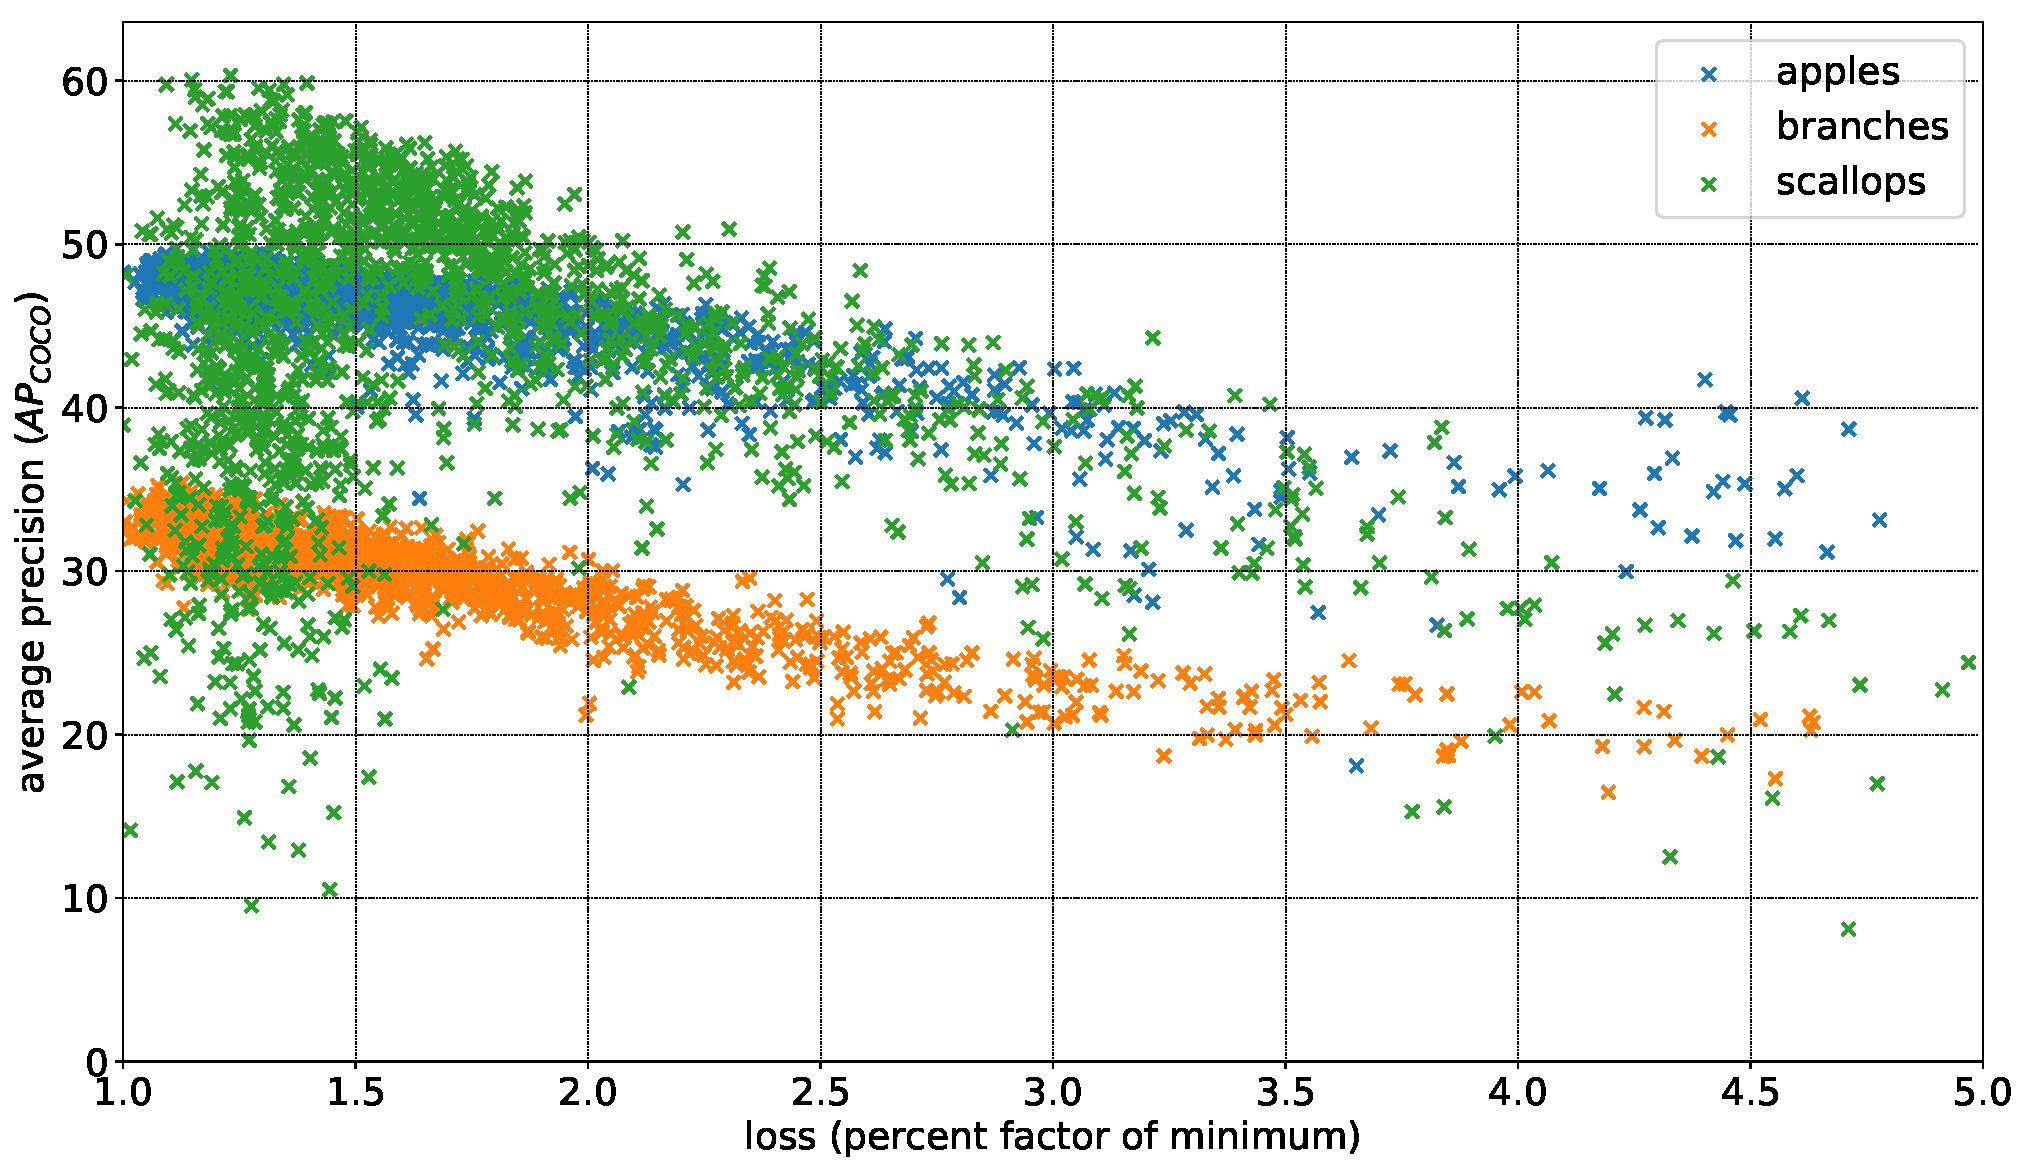
\includegraphics[width=1.0\linewidth]{charts/training/lr_schedule/scatter_loss_ap.pdf}
  \caption{Correlation between loss function and validation $AP_{COCO}$ for three different datasets across 6 repeated training runs (non incremental case)}  
  \label{fig:scatter_loss_ap}
\end{figure}

The tests showed a considerable amount of noise, especially for the \emph{scallop} dataset, so it was repeated six times to attempt to distil anything useful from it. Figure~\ref{fig:scatter_loss_ap} shows the differences in variability between the three datasets used. In particular, for the \emph{scallop} case, the correlation between loss and validation \gls{AP} is noisy, possibly from either overfitting or inconsistent annotations.

\begin{figure}[htb]
\centering
\begin{subfigure}[t]{0.5\linewidth}
  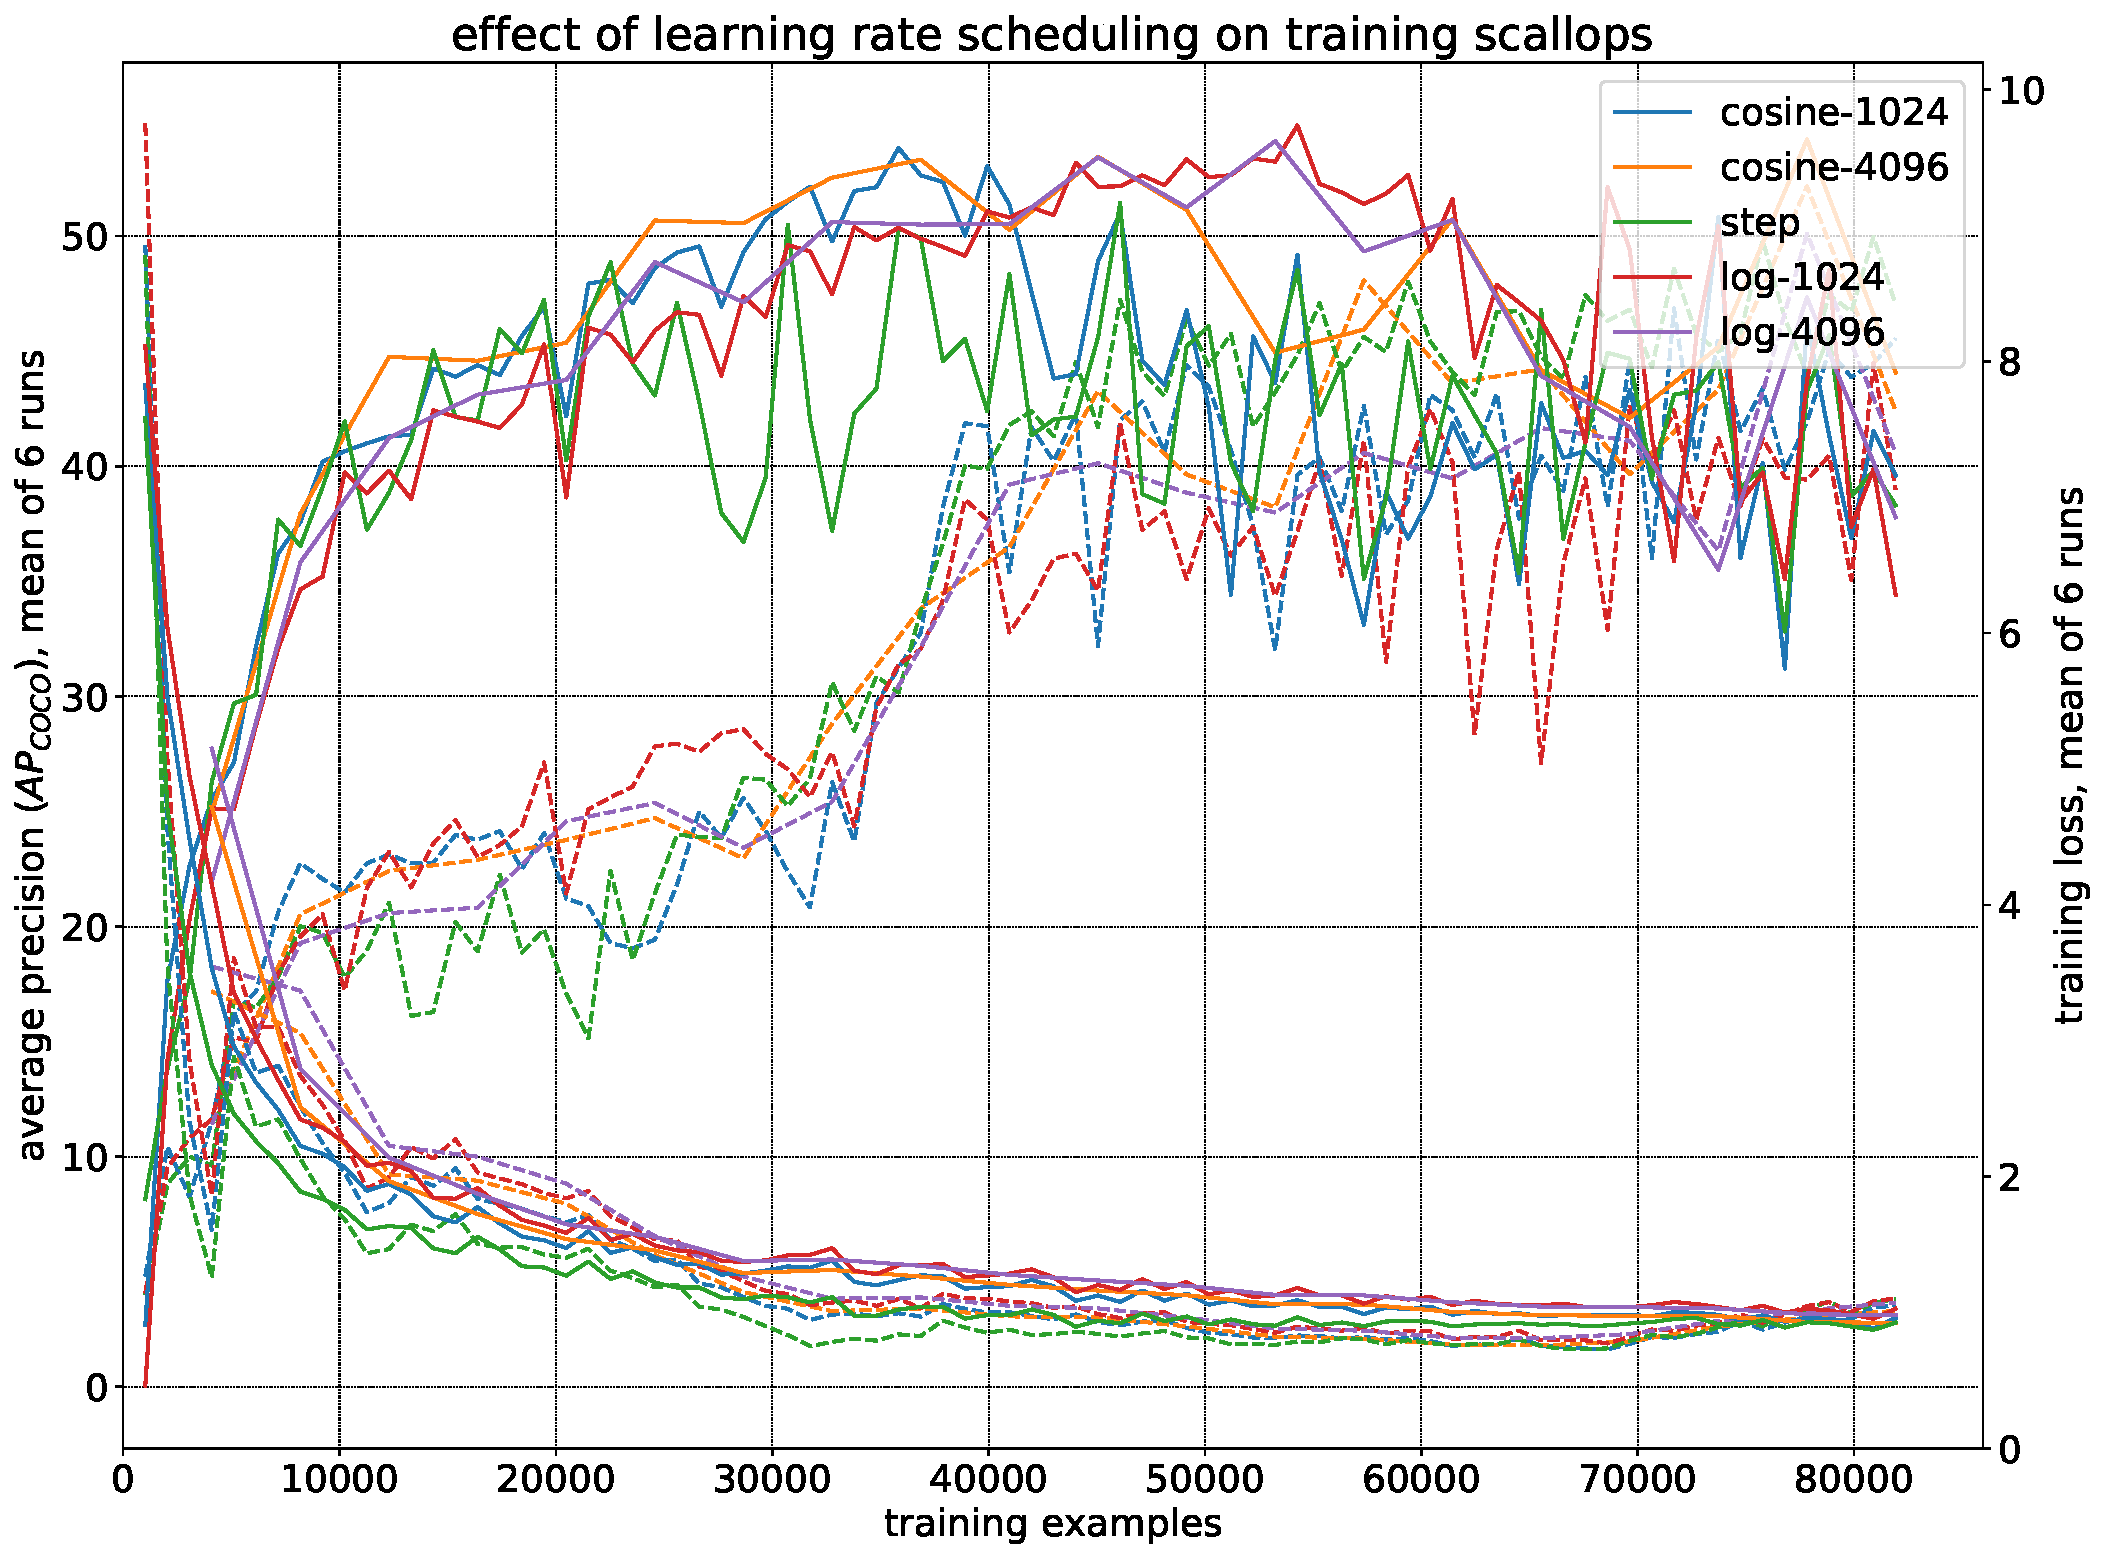
\includegraphics[width=1.0\linewidth]{charts/training/lr_schedule/scallops.pdf}
  \caption{}
\end{subfigure}%
\begin{subfigure}[t]{0.5\linewidth}
  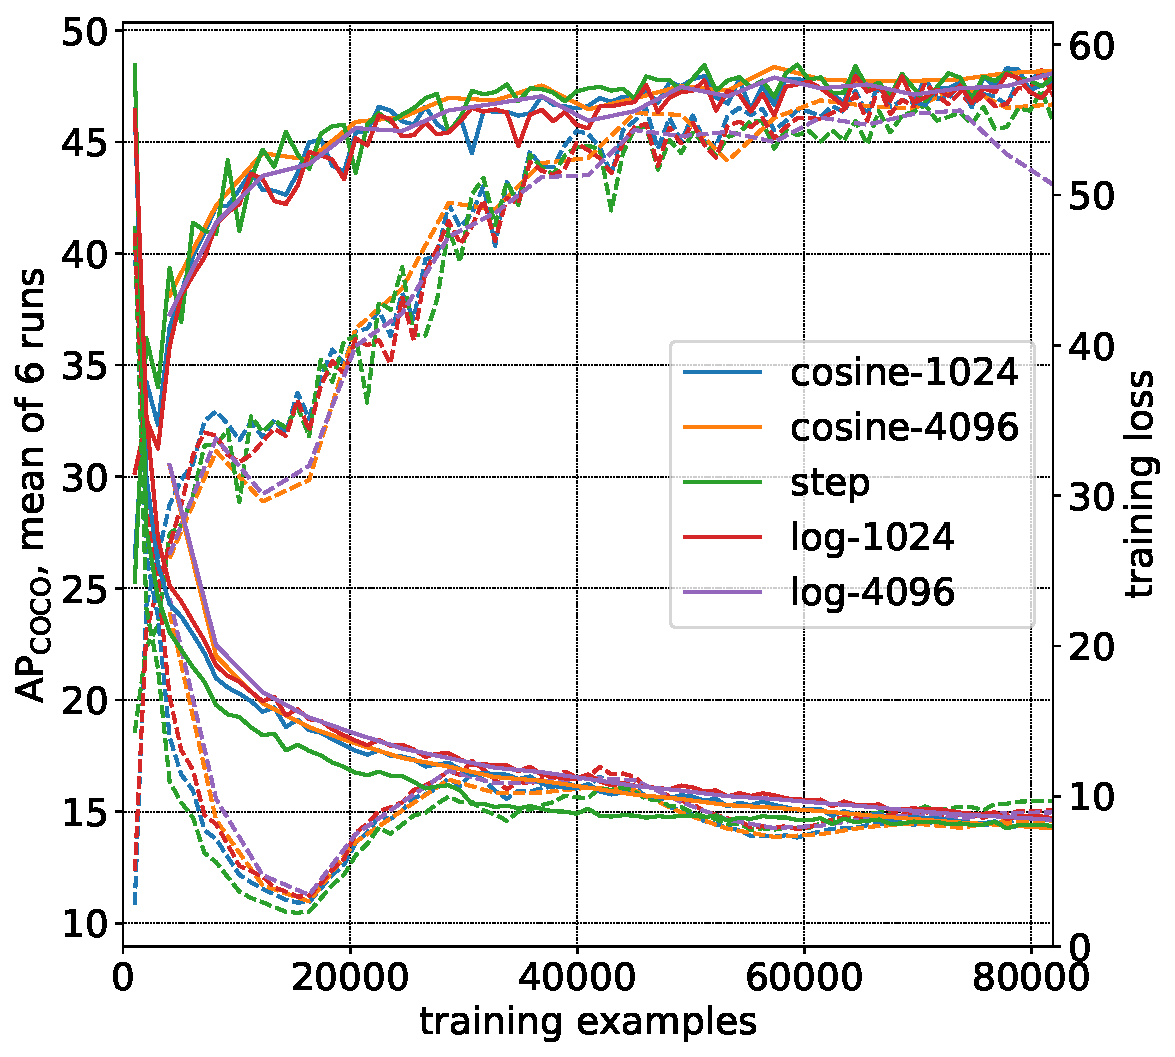
\includegraphics[width=1.0\linewidth]{charts/training/lr_schedule/apples.pdf}
  \caption{}
\end{subfigure}
  \caption{Training of (a) \emph{scallop} (b) $apples^1$. The bottom lines show the loss function and the top show validation $AP_{COCO}$}  
  \label{fig:datasets_lr}
\end{figure}

Figure~\ref{fig:datasets_lr} shows training runs for $apples^1$ and \emph{scallop} datasets, the pattern for \emph{branches} was very similar to $apples^1$. A noticeable pattern can be seen in the incremental case where the validation \gls{AP} increases positively with the number of examples used in training, showing that the factor limiting the accuracy is the size of the dataset (the number of annotated images so far).

There seems to be little difference of note between learning rate schedules in terms of either the validation accuracy or the amount the loss function is reduced. In the beginning, the \emph{incremental} loss is reduced much faster than the \emph{full} case, because it can fit the small number of examples much better. The constant learning rate reduces the loss better in the early part of the training process, but towards the end, there seems little difference between the methods. 

Further study will be required on larger datasets to determine if this is something useful to persevere with, but from this small experiment alone it seems that using the cyclical learning rate is less important than was expected. Another alternative is to assign individual learning rates to images or object instances which anneal as they are seen more times by the training process.

\section{Sensitivity to noise and systematic bias}
\label{sec:noise_sensitivity}

In this experiment, I examine how tolerant the object detector is to two factors: (a) random noisy annotations, (b) systematic bias and combinations of the two. All human annotation contains a certain amount of noise as well as a bias which varies from person to person and activity to activity, so it is expected an object detector can tolerate a certain amount of labelling noise in its training data. 

A \gls{VBA} based system by nature of using an object detector trained on noisy inputs, will therefore not produce entirely accurate localised predictions. The hope is that such a system will eventually produce localisations that are \emph{good enough}, in order that predictions from the object detector can be accepted without taking up valuable annotator time. In this experiment, I aim to quantify how noise degrades performance, and therefore establish some idea of what guideline for the level of precision is required during annotation.

In Chapter~\ref{chap:annotation}, I examine from an annotation perspective, what was considered acceptable during the annotation of these datasets by looking at the distributions of corrected annotations and how they compare to the predictions supplied by the model. 

\subsection{Method}

I added noise and systematic bias to five different datasets, covering a range of parameters (resolutions, object sizes, instance counts), where validation accuracy was highest among the datasets created in this work. These five are: \emph{branches}, $apples^2$ ($50\%$ scale), \emph{scott base}, \emph{seals} ($50\%$ scale) and \emph{penguins} ($50\%$ scale). Three datasets are down-sampled to save time. Two datasets are not down-sampled: one of them because the resolution is already low, and the other because the objects are already very small for the object detector.

Noise is added by randomly moving the box centre and randomly scaling the box size. The box centre ($c_x$, $c_y$) is moved as a proportion of the size of the box to become ($\hat{c}_x$, $\hat{c}_y$), and the width and height ($w$ and $h$) of the box are multiplied by translation ($t_x$, $t_y$) and scaling ($s_x$, $s_y$) factors sampled from a normal distribution. The standard deviation of the distribution $\sigma$ controls the magnitude of the translation and scaling. 

Systematic bias is added as a proportion of box width and height also, controlled by a parameter factor $\Delta$; in this experiment, the box is always moved up and to the right. The final transformed box is then specified by $\hat{c}_x$, $\hat{c}_y$, $\hat{w}$, $\hat{h}$ according to equation~\ref{eq:noisy_box}. 

\begin{equation}
\begin{split}
    s_w, s_h \sim \mathcal{N}(1,\,\sigma^{2})\\
    t_x, t_y \sim \mathcal{N}(0,\,\sigma^{2})\\
    \hat{c}_x = c_x + (\Delta + t_x) w\\
    \hat{c}_y = c_y + (\Delta + t_y) h\\
    \hat{w} = s_x w\\
    \hat{h} = s_h h\\
\end{split}
\label{eq:noisy_box}
\end{equation}

The noise is consistent throughout training as opposed to being added as a form of data label augmentation. Systematic offset factor $\Delta$ is also added to the validation set, assuming such a form of error would be uniform across the data. With an offset, the challenge for the object detector is if the detector can adapt its estimations when the real object in question is translated with respect to the centres in the feature map of the receptive field. Noise, on the other hand, is added only to the training data and not to the validation data as adding noise changes the mean of box centre or size (on average).

The object detector is trained for $40$ epochs in five different configurations of noise and systematic offset: $\sigma \in [0\%, 4\%, 8\%, 16\%, 32\%]$ and $\Delta \in [0\%, 4\%, 8\%, 16\%, 32\%]$. Object detectors are trained with standard parameters for each dataset (except the three which are trained at $50\%$ scale), and the impact of the noise and systematic offset is measured by looking at the peak validation \gls{AP} at different thresholds.

After noticing overfitting occurring in noisy cases, the set of experiments were repeated with reduced training data to examine how noise affected generalisation. I used two low training data scenarios, firstly at $25\%$ of training examples, then at $6.25\%$.

The amount of noise and the resulting mean \gls{IOU}s with the original box can be seen visually in Figure~\ref{fig:noisy_training}. It can be seen that the levels of noise and systematic offset, both have approximately the same mean \gls{IOU}s with respect to the original boxes for the particular level of offset or bias.

\begin{figure}[phbt!]
\centering
\begin{subfigure}[t]{0.5\linewidth}
  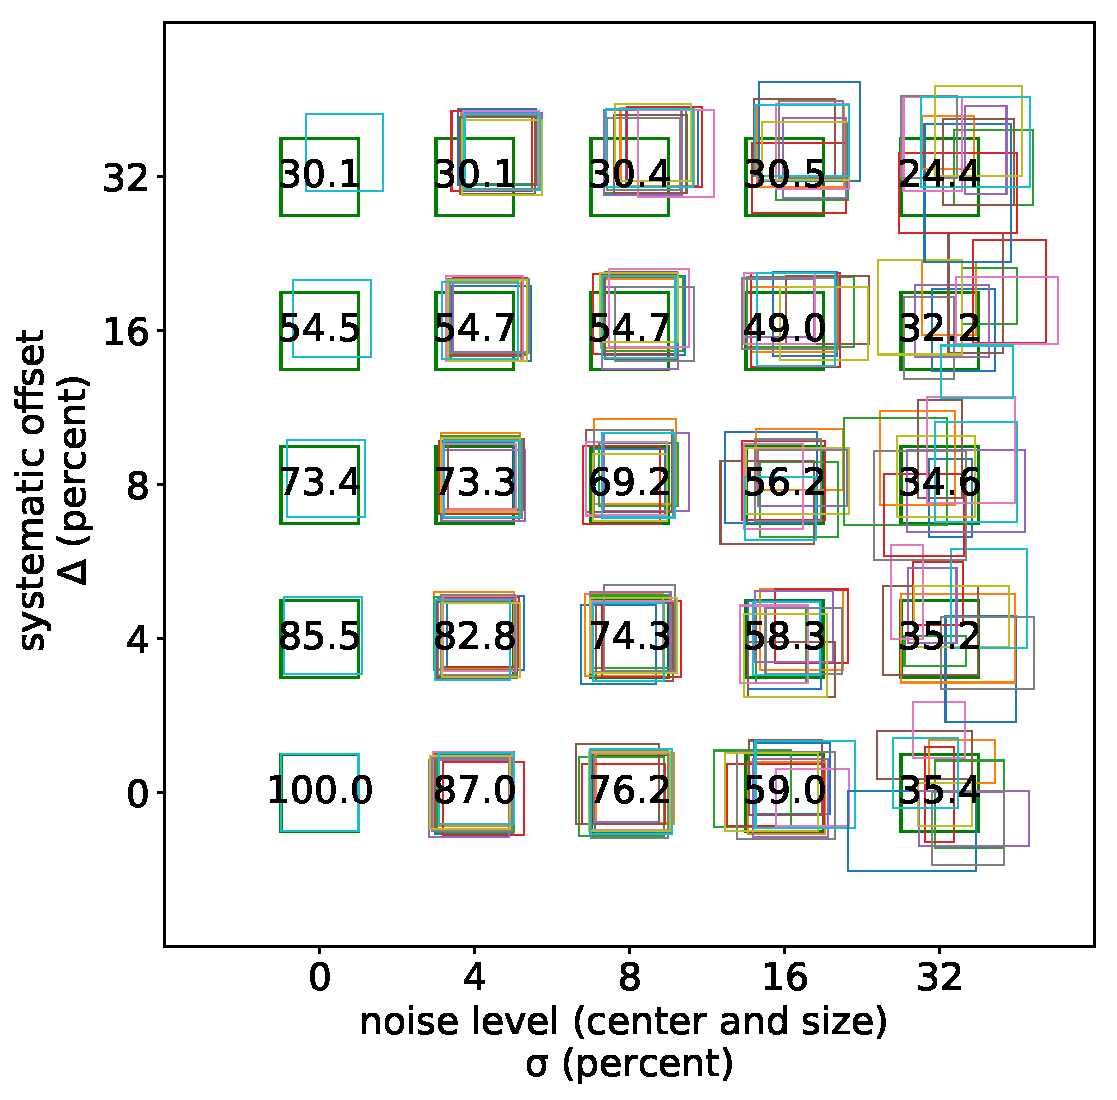
\includegraphics[width=1.0\linewidth]{charts/training/noisy_boxes.pdf}
  \caption{}
\end{subfigure}%
\begin{subfigure}[t]{0.5\linewidth}
  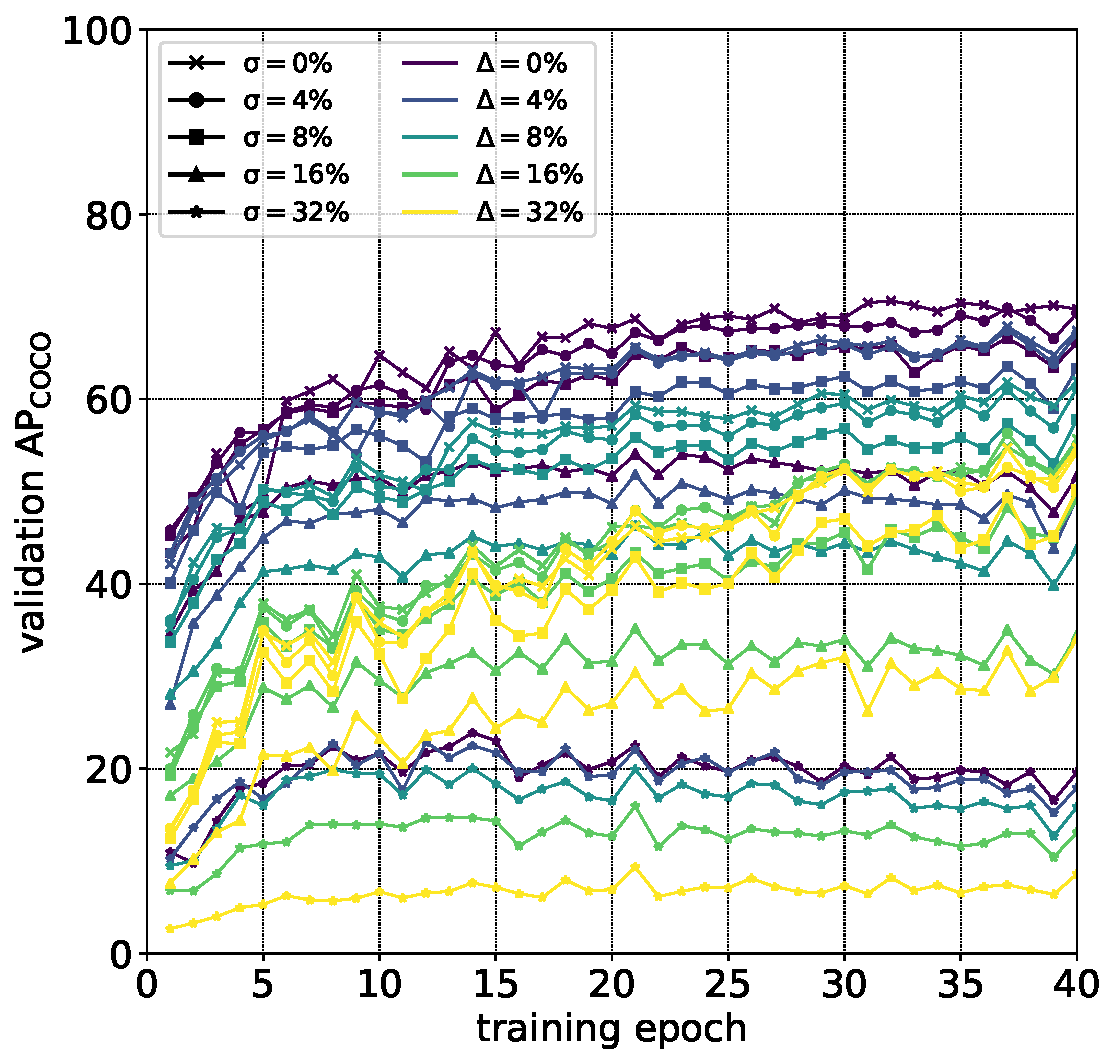
\includegraphics[width=1.0\linewidth]{charts/training/noise_training.pdf}
  \caption{100\% training images}
\end{subfigure}
\begin{subfigure}[t]{0.5\linewidth}
  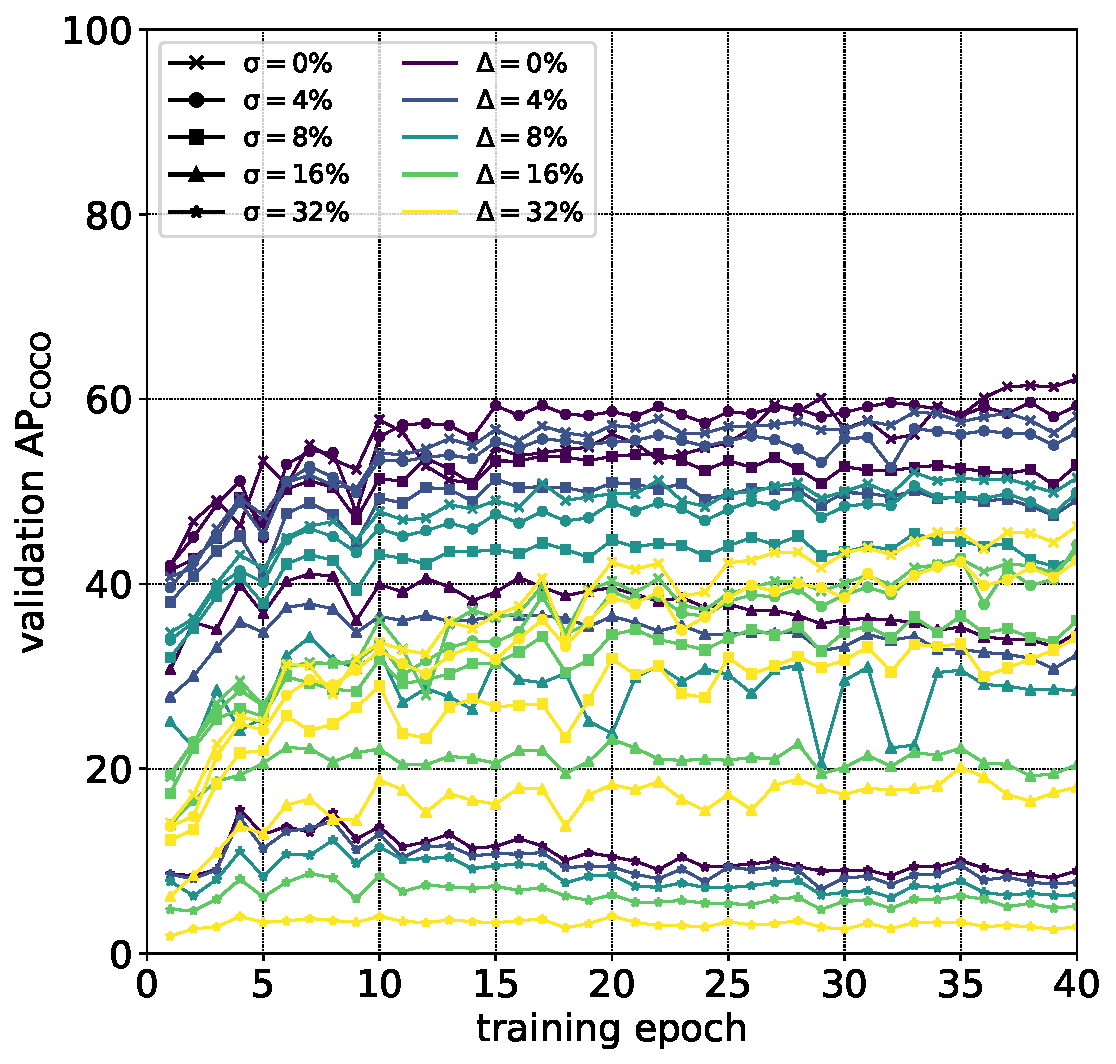
\includegraphics[width=1.0\linewidth]{charts/training/noise_4_training.pdf}
  \caption{25\% training images}
\end{subfigure}%
\begin{subfigure}[t]{0.5\linewidth}
  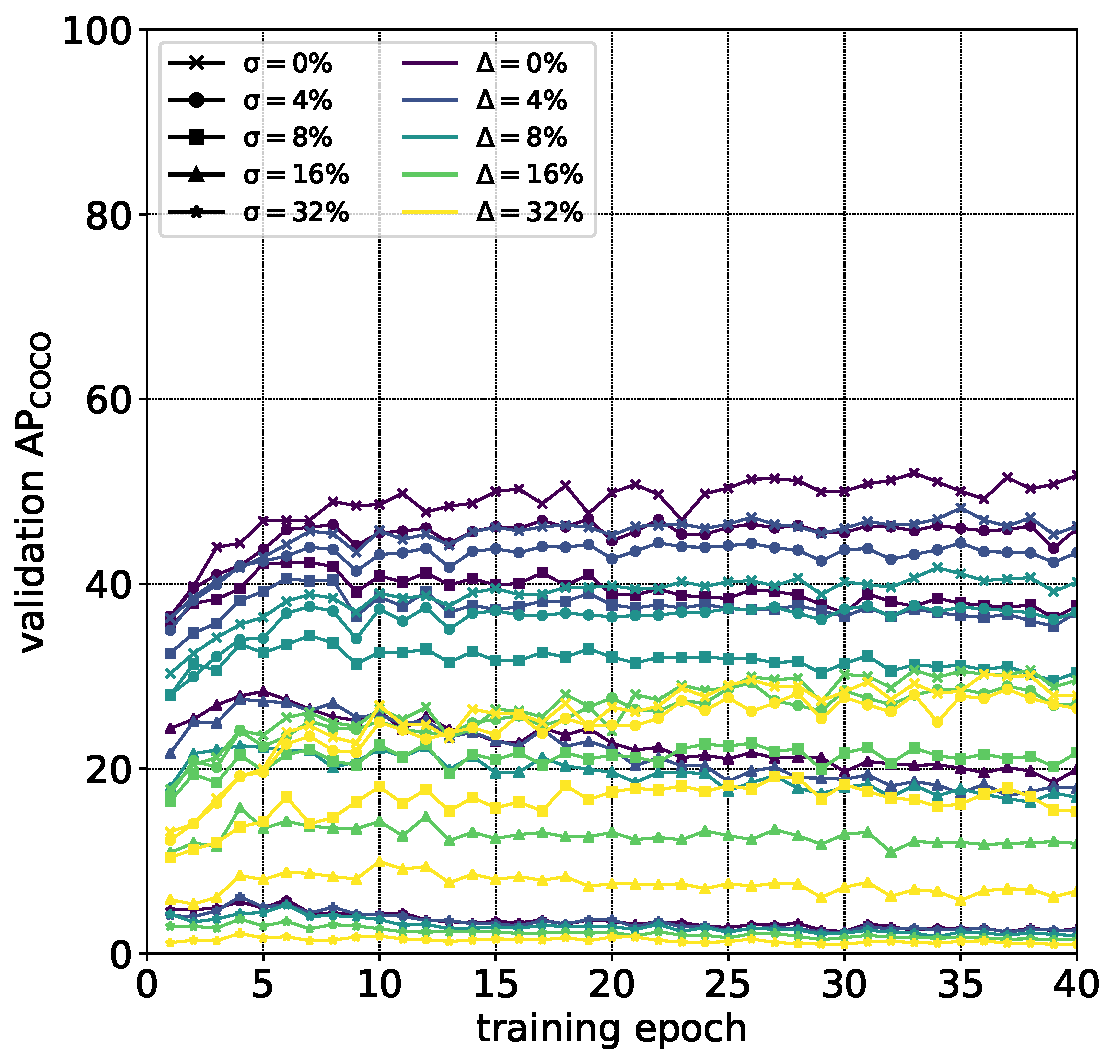
\includegraphics[width=1.0\linewidth]{charts/training/noise_16_training.pdf}
  \caption{6.25\% training images}
\end{subfigure}
  \caption{ (a) Samples of the different noise and systematic bias added, showing reference box with 10 samples; overlaid with the mean \gls{IOU} for that condition. (b), (c), (d) $AP_{COCO}$ validation after training with with varying noise and systematic bias added, and varying training set size. Average of training runs of 5 different datasets, at half-resolution: \emph{seals}, $apples^2$ and \emph{penguins}; at full-resolution: \emph{scott base}, \emph{branches}}
  \label{fig:noisy_training}
\end{figure}

\subsection{Results and discussion}

\begin{table}[phbt!]
\caption {Best validation $AP_{50}$, $AP_{75}$, with different levels of added noise ($\sigma$) and systematic bounding box offset ($\Delta$) and at different sizes of training data. Baseline ($\sigma=0$, $\Delta=0$) in each case shown as absolute value in bold, other cases shown as percent change. Mean and standard deviation of training runs of 5 different datasets, at half-resolution: \emph{seals}, $apples^2$ and \emph{penguins}; at full-resolution: \emph{scott base}, \emph{branches}.}
\label{tab:noise_table}


\begin{subfigure}[b]{\linewidth}
\caption{$100\%$ training data}
\begin{adjustbox}{max width=\textwidth}
\begin{tabular}{ll|lllll}
 & & $\Delta=0\%$              & $\Delta=4\%$              & $\Delta=8\%$              & $\Delta=16\%$              & $\Delta=32\%$              \\

\toprule
\multirow{2}{*}{\STAB{\rotatebox[origin=c]{90}{$AP_{50}$}}}
 & $\sigma=0\%$  & $\mathbf{95.1\pm2.7}$  & $-0.6\pm0.6\%$  & $-0.7\pm0.7\%$  & $-2.8\pm2.1\%$  & $-10.1\pm10.6\%$ \\
 & $\sigma=4\%$  & $-0.3\pm0.6\%$  & $-0.4\pm0.6\%$  & $-1.3\pm1.4\%$  & $-2.8\pm1.7\%$  & $-10.4\pm10.3\%$ \\
 & $\sigma=8\%$  & $-1.1\pm0.8\%$  & $-1.3\pm1.7\%$  & $-2.4\pm1.5\%$  & $-4.0\pm2.3\%$  & $-12.6\pm9.8\%$  \\
 & $\sigma=16\%$ & $-6.9\pm4.7\%$  & $-8.4\pm5.3\%$  & $-8.0\pm4.4\%$  & $-10.2\pm3.7\%$ & $-23.8\pm11.7\%$ \\
 & $\sigma=32\%$ & $-32.6\pm6.8\%$ & $-32.1\pm7.1\%$ & $-36.1\pm4.4\%$ & $-42.2\pm4.8\%$ & $-61.5\pm6.6\%$ \\

\toprule
\multirow{2}{*}{\STAB{\rotatebox[origin=c]{90}{$AP_{75}$}}}
 & $\sigma=0\%$  & $\mathbf{84.0\pm8.5}$   & $-2.7\pm1.5\%$   & $-9.1\pm3.4\%$   & $-27.3\pm21.5\%$ & $-24.1\pm17.0\%$ \\
 & $\sigma=4\%$  & $-2.1\pm1.1\%$   & $-2.9\pm1.1\%$   & $-10.5\pm4.0\%$  & $-26.8\pm21.0\%$ & $-24.3\pm15.8\%$ \\
 & $\sigma=8\%$  & $-7.5\pm7.7\%$   & $-8.6\pm5.2\%$   & $-17.0\pm7.7\%$  & $-42.5\pm14.9\%$ & $-32.7\pm12.7\%$ \\
 & $\sigma=16\%$ & $-23.8\pm16.4\%$ & $-30.1\pm16.7\%$ & $-42.4\pm14.3\%$ & $-71.0\pm8.9\%$  & $-63.4\pm11.7\%$ \\
 & $\sigma=32\%$ & $-81.3\pm7.2\%$  & $-83.4\pm6.0\%$  & $-86.6\pm3.2\%$  & $-94.9\pm2.5\%$  & $-97.0\pm1.3\%$  \\
\bottomrule
\end{tabular}
\end{adjustbox}
\label{tab:noise_table_100}
\end{subfigure}
\begin{subfigure}[b]{\linewidth}
\caption{$25\%$ training data}
\begin{adjustbox}{max width=\textwidth}
\begin{tabular}{ll|lllll}
 & & $\Delta=0\%$              & $\Delta=4\%$              & $\Delta=8\%$              & $\Delta=16\%$              & $\Delta=32\%$              \\

\toprule
\multirow{2}{*}{\STAB{\rotatebox[origin=c]{90}{$AP_{50}$}}}
& $\sigma=0\%$ & $\mathbf{ 86.9\pm7.7 }$ & $-0.4\pm1.4\%$ & $-2.0\pm1.7\%$ & $-7.2\pm6.2\%$ & $-18.3\pm16.5\%$ \\ 
& $\sigma=4\%$ & $0.4\pm2.6\%$ & $0.5\pm1.5\%$ & $-1.6\pm2.5\%$ & $-8.1\pm7.4\%$ & $-19.8\pm14.8\%$ \\ 
& $\sigma=8\%$ & $-1.2\pm1.3\%$ & $-1.9\pm1.7\%$ & $-3.1\pm2.7\%$ & $-9.1\pm7.6\%$ & $-23.1\pm16.7\%$ \\ 
& $\sigma=16\%$ & $-9.0\pm7.7\%$ & $-9.2\pm6.6\%$ & $-11.9\pm9.1\%$ & $-20.4\pm10.9\%$ & $-38.3\pm12.6\%$ \\ 
& $\sigma=32\%$ & $-41.3\pm8.6\%$ & $-43.5\pm7.8\%$ & $-46.3\pm8.1\%$ & $-55.8\pm7.1\%$ & $-75.6\pm3.8\%$ \\ 


\toprule
\multirow{2}{*}{\STAB{\rotatebox[origin=c]{90}{$AP_{75}$}}}
& $\sigma=0\%$ & $\mathbf{ 72.8\pm16.4 }$ & $-6.3\pm6.4\%$ & $-18.6\pm9.0\%$ & $-39.5\pm17.5\%$ & $-29.2\pm19.2\%$ \\ 
& $\sigma=4\%$ & $-6.1\pm5.0\%$ & $-8.7\pm7.4\%$ & $-24.7\pm11.6\%$ & $-38.2\pm20.8\%$ & $-34.8\pm17.6\%$ \\ 
& $\sigma=8\%$ & $-19.1\pm17.8\%$ & $-21.7\pm14.8\%$ & $-33.2\pm14.7\%$ & $-56.3\pm14.8\%$ & $-51.1\pm18.9\%$ \\ 
& $\sigma=16\%$ & $-39.5\pm24.5\%$ & $-48.3\pm24.8\%$ & $-59.3\pm19.5\%$ & $-82.8\pm12.6\%$ & $-76.1\pm15.3\%$ \\ 
& $\sigma=32\%$ & $-86.9\pm7.9\%$ & $-87.2\pm9.1\%$ & $-92.3\pm5.5\%$ & $-97.6\pm1.4\%$ & $-98.7\pm0.5\%$ \\ 
\bottomrule
\end{tabular}
\end{adjustbox}
\label{tab:noise_table_4}
\end{subfigure}
\begin{subfigure}[b]{\linewidth}
\caption{$6.25\%$ training data}
\begin{adjustbox}{max width=\textwidth}
\begin{tabular}{ll|lllll}
 & & $\Delta=0\%$              & $\Delta=4\%$              & $\Delta=8\%$              & $\Delta=16\%$              & $\Delta=32\%$              \\

\toprule
\multirow{2}{*}{\STAB{\rotatebox[origin=c]{90}{$AP_{50}$}}}
& $\sigma=0\%$ & $\mathbf{ 75.1\pm23.2 }$ & $-3.9\pm7.7\%$ & $-4.2\pm6.5\%$ & $-15.4\pm11.8\%$ & $-31.7\pm19.6\%$ \\ 
& $\sigma=4\%$ & $-6.7\pm9.9\%$ & $-2.1\pm3.2\%$ & $-4.0\pm2.0\%$ & $-15.7\pm14.1\%$ & $-31.6\pm19.8\%$ \\ 
& $\sigma=8\%$ & $-2.2\pm2.7\%$ & $-4.6\pm6.1\%$ & $-8.8\pm9.1\%$ & $-18.9\pm10.1\%$ & $-42.8\pm17.6\%$ \\ 
& $\sigma=16\%$ & $-18.7\pm9.8\%$ & $-21.0\pm15.5\%$ & $-21.9\pm8.3\%$ & $-30.2\pm11.6\%$ & $-58.8\pm12.7\%$ \\ 
& $\sigma=32\%$ & $-68.6\pm12.2\%$ & $-70.8\pm10.6\%$ & $-71.6\pm8.4\%$ & $-76.6\pm9.0\%$ & $-87.1\pm5.3\%$ \\ 

\toprule
\multirow{2}{*}{\STAB{\rotatebox[origin=c]{90}{$AP_{75}$}}}
& $\sigma=0\%$ & $\mathbf{ 61.5\pm26.7 }$ & $-8.8\pm6.4\%$ & $-29.3\pm9.8\%$ & $-55.1\pm13.6\%$ & $-46.9\pm14.1\%$ \\ 
& $\sigma=4\%$ & $-10.1\pm5.0\%$ & $-16.7\pm8.9\%$ & $-40.6\pm14.1\%$ & $-58.7\pm19.1\%$ & $-51.8\pm14.4\%$ \\ 
& $\sigma=8\%$ & $-25.7\pm15.2\%$ & $-32.9\pm18.1\%$ & $-51.4\pm12.9\%$ & $-76.8\pm10.9\%$ & $-76.5\pm6.7\%$ \\ 
& $\sigma=16\%$ & $-63.7\pm20.6\%$ & $-67.9\pm23.2\%$ & $-77.0\pm15.2\%$ & $-92.4\pm7.7\%$ & $-93.4\pm5.1\%$ \\ 
& $\sigma=32\%$ & $-97.4\pm1.8\%$ & $-97.2\pm1.8\%$ & $-98.0\pm1.2\%$ & $-98.7\pm0.7\%$ & $-99.6\pm0.2\%$ \\ 

\bottomrule
\end{tabular}
\end{adjustbox}
\label{tab:noise_table_16}
\end{subfigure}
\end{table}


The impact in terms of degradation of object detection performance can be seen in Table~\ref{tab:noise_table}, shown as the reduction in performance from the baseline zero noise and zero offset cases (shown as the absolute value, in bold). Two matching thresholds are shown, a relaxed matching threshold $AP_{50}$ and at strict matching threshold $AP_{75}$, which includes boxes which are closer to localisation error acceptable to human verification (see Section~\ref{sec:verification_threshold}). 

The object detector at a relaxed matching threshold $AP_{50}$ seems robust to a small amount of noise and systematic offset; less than $8\%$ offset or noise shows only a small impact on $AP_{50}$ degradation in each case, even in the low data scenarios. For the full amount of data, $AP_{50}$ is only degraded $10\%$ at $\sigma = 16\%, \Delta = 16\%$, yet in the same case $AP_{75}$ is reduced by $71\%$.

For the full amount of training data, $AP_{75}$ is also robust to a small amount of noise or offset, roughly $2\%$ degradation of performance for $4\%$ noise or offset. Human variation of box annotation in \cite{Papadopoulos2017} was reported as a mean \gls{IOU} of 88, which corresponds to the noise case of $\sigma = 4\%$. At that noise level, performance degradation is minimal, even for a strict matching criterion, degrading $AP_{75}$ by around $2\%$. Keep in mind that these datasets were human annotated to begin with, so the noise added is extra noise.

Sensitivity to noise and systematic offset is seen to increase significantly with less training data. At $\sigma=4\%$, a level of noise similar to a human annotator, $AP_{75}$ is degraded by $2.1\%$ at $100\%$ images, increasing to $6.1\%$ at $25\%$ images and $10.1\%$ at $6.25\%$ of the training images. This increased sensitivity can be seen across the range of noise and offset, and at $6.25\%$ of the images, $AP_{50}$ is degraded approximately double the amount compared to at $25\%$ of the images.

Overfitting can be seen to occur at higher levels and offset in Figure~\ref{fig:noisy_training}, where the validation scores peak and start to degrade gradually with further training. The trajectory of validation accuracy can be seen to peak early and slowly fall off in the noisy cases for all three levels of training data, however in the low data scenarios, especially with only $6.25\%$ training examples, even a small amount of noise causes the accuracy to decline as training continues. Adding an offset seems to have a different effect, where accuracy is substantially degraded to begin with, but slowly improves with additional training.

Noise at $\sigma = 32\%$ was much worse in all cases, but this can be considered a special case. Using a normally distributed scaling at high noise values such as $\sigma = 32\%$ was probably an incorrect choice, as it can result in boxes of significantly different aspect ratio to the original box. Adding noise to the corner positions may have been more appropriate at this high noise level.

In Chapter~\ref{chap:annotation}, I attempt to quantify the implicit human localisation threshold for correcting errors using real-world annotations with the \gls{VBA} tool. During the development of the object detector, a localisation bug caused such a systematic localisation bias during use for a counting task. Despite counting a very similar number of instances, the object detection performance on the final set of annotations can be seen to be significantly degraded (differences between annotators could also be a factor).

\subsection{Future work}

An interesting aspect, a study for the future, would be to look at the fixed point. If an object detector is fed back its outputs, how does the error change over iterations depending on input noise? Does a systematic bias amplify itself with iteration? Then, study how error correction (for example from a \gls{VBA} system) is necessary to (a) break even, and (b) improve object detection performance. A user would complement these experiments by examining how much noise and bias propagate to final annotations.

\subsection{Summary}

Overall it can be seen (and is not surprising) that noise and systematic offset are much more problematic for strict matching criteria. So, if the goal is to annotate a lot of data fast (but not accurately), using a \gls{VBA} system, that has a fast and approximate strategy for annotation, may be successful if all that is required is more approximate localisation. However, with less training images (such as near the start of annotation), the object detector becomes much more sensitive to both noise and systematic offset. At higher noise levels, this can be seen to be further compounded by overfitting. It would seem prudent to focus on higher accuracy annotation, at least to begin with, both from an annotator's perspective and a tool-author's perspective, to facilitate this.

\section {Summary}

This chapter described the object detector used behind the annotation tool, parameters used, and proposed some modifications to the standard practice in order to better suit its use for the purposes of assisted image annotation including high-resolution training and inference, cyclical learning rates for incremental training, non shared classifier sub-networks and non normalised loss function. I performed some experiments to attempt to validate some of these ideas and test assumptions made during the design of the annotation tool.

I demonstrated an approach to training and inference for high-resolution images. By training with image crops, a higher accuracy is possible using the full image resolution (at the expense of training time, however during annotation, time is plentiful). In each case, using larger crop sizes proved better, with smaller crop sizes being less accurate and destabilising training. Two different methods of inference at high-resolution were tested, one by using the property of the \gls{FCN}, the other by tiling; both were found to be approximately equal, with one trading off time and the other trading off memory usage.

Training with cyclical learning rates was shown to perhaps be less critical than assumed, at least in the experimental conditions used here. There existed little difference between training with a constant learning rate and the various forms of cyclical learning rates. Testing with incrementally adding training images showed the generalisation was limited by the number of examples added.

I performed an investigation of the impact of annotation localisation noise, as well as systematic localisation error. The results show that training with many images is robust to a small amount of localisation error, however, with fewer images the sensitivity is much higher, leading to degradation of performance with even a small amount of noise; this suggests a focus on accurate object localisation is important, especially near the beginning of annotation, for both annotator and tool author.



